%; whizzy chapter
% -initex iniptex -latex platex -format platex -bibtex jbibtex -fmt fmt
% $B0J>e(B whizzytex $B$r;HMQ$9$k>l9g$N@_Dj!#(B

%     Tokyo Debian Meeting resources
%     Copyright (C) 2010 Junichi Uekawa

%     This program is free software; you can redistribute it and/or modify
%     it under the terms of the GNU General Public License as published by
%     the Free Software Foundation; either version 2 of the License, or
%     (at your option) any later version.

%     This program is distributed in the hope that it will be useful,
%     but WITHOUT ANY WARRANTY; without even the implied warranty of
%     MERCHANTABILITY or FITNESS FOR A PARTICULAR PURPOSE.  See the
%     GNU General Public License for more details.

%     You should have received a copy of the GNU General Public License
%     along with this program; if not, write to the Free Software
%     Foundation, Inc., 51 Franklin St, Fifth Floor, Boston, MA  02110-1301 USA

%  preview (shell-command (concat "evince " (replace-regexp-in-string "tex$" "pdf"(buffer-file-name)) "&"))
% $B2hA|%U%!%$%k$r=hM}$9$k$?$a$K$O(Bebb$B$rMxMQ$7$F(Bboundingbox$B$r:n@.!#(B
%(shell-command "cd image201003; ebb *.png")

%%$B$3$3$+$i%X%C%@3+;O!#(B

\documentclass[mingoth,a4paper]{jsarticle}
\usepackage{monthlyreport}
\usepackage{wrapfig}
\usepackage{amsmath}

% $BF|IU$rDj5A$9$k!"Kh7nJQ$o$j$^$9!#(B
\newcommand{\debmtgyear}{2010}
\newcommand{\debmtgmonth}{3}
\newcommand{\debmtgdate}{20}
\newcommand{\debmtgnumber}{62}

\begin{document}
\begin{titlepage}
\thispagestyle{empty}

% $B%?%$%H%k%Z!<%8(B:$BJT=8I,MW$JItJ,$O:G=i$N%^%/%m$KHt$P$9$3$H(B

\vspace*{-2cm}
$BBh(B\debmtgnumber{}$B2s(B $BEl5~%(%j%"(B Debian $BJY6/2q;qNA(B\\
\hspace*{-2cm}

\includegraphics[width=210mm]{image201003/debsen.eps}\\
\hfill{}\debmtgyear{}$BG/(B\debmtgmonth{}$B7n(B\debmtgdate{}$BF|(B\\
%\vspace*{-2.4cm}

\rotatebox{10}{\fontsize{32}{32} {\gt $BFC=8(B1: $B%K%e!<%i%k%M%C%H%o!<%/FC=8(B}}

\rotatebox{10}{\fontsize{32}{32} {\gt $BFC=8(B2: man-db$B$K$O$^$C$F$_$?(B} }

\vspace*{-2cm}
\hfill{}
\includegraphics[height=6cm]{image200502/openlogo-nd.eps}
\end{titlepage}

\dancersection{Introduction}{$B>e@n(B $B=c0l(B}

\begin{multicols}{2}
 
 
 $B:#7n$N(BDebian$BJY6/2q$X$h$&$3$=!#$3$l$+$i(BDebian$B$N@$3&$K$"$7$rF'$_F~$l$k$H(B
 $B$$$&J}$b!"$9$G$K$I$C$W$j$H$D$+$C$F$$$k$H$$$&J}$b!"7n$K0l2s(BDebian$B$K$D$$(B
 $B$F8l$j$^$;$s$+!)(B

 Debian$BJY6/2q$NL\E*$O2<5-$G$9!#(B

 \begin{itemize}
 \item \underline{Debian Developer} ($B3+H/<T(B)$B$N0i@.!#(B
 \item $BF|K\8l$G$N!V(B\underline{$B3+H/$K4X$9$k>pJs(B}$B!W$r@0M}$7$F$^$H$a!"%"%C%W%G!<%H$9$k!#(B
 \item \underline{$B>l(B}$B$NDs6!!#(B
 \begin{itemize}
  \item $BIaCJ$P$i$P$i$J>l=j$K$$$k?M!9$,(B face-to-face $B$G=P2q$($k>l$rDs6!(B
	$B$9$k!#(B
  \item Debian $B$N$?$a$K$J$k$3$H$r8l$k>l$rDs6!$9$k!#(B
  \item Debian$B$K$D$$$F8l$k>l$rDs6!$9$k!#(B
 \end{itemize}
 \end{itemize}		

 Debian$B$NJY6/2q$H$$$&$3$H$G5f6KE*$K$O;22C<TA40w$,(BDebian Package$B$r$,$j$,$j(B
 $B$H:n$k%9!<%Q!<%O%C%+!<$K$J$C$?;Q$rLQA[$7$F$$$^$9!#>pJs$N6&M-!&3hMQ$rDL$7(B
 $B$F(B Debian$B$N:#8e$NG=F0E*$JE83+$X$NEZBf$H$7$F!"!V>l!W$H$7$F$N6u4V$rDs6!$9(B
 $B$k$N$,L\E*$G$9!#(B

\end{multicols}

\newpage

\begin{minipage}[b]{0.2\hsize}
 \definecolor{titleback}{gray}{0.9}
 \colorbox{titleback}{\rotatebox{90}{\fontsize{80}{80} {\gt $B%G%S%"%sJY6/2q(B} }}
\end{minipage}
\begin{minipage}[b]{0.8\hsize}
\hrule
\vspace{2mm}
\hrule
\tableofcontents
\vspace{2mm}
\hrule
\end{minipage}

\dancersection{$B;vA02]Bj(B}{$B>e@n(B $B=c0l(B}

$B:#2s$N;vA02]Bj$O0J2<$G$9(B:

\begin{enumerate}
 \item $B9%$-$JF|K\8l(BMan$B%Z!<%8(B
 \item $B%K%e!<%i%k%M%C%H%o!<%/$G2r7h$G$-$kLdBj(B
\end{enumerate}

$B$3$N2]Bj$KBP$7$FDs=P$$$?$@$$$?FbMF$O0J2<$G$9!#(B


% this is a prework file.


\dancersection{$B:G6a$N(BDebian$B4XO"$N%_!<%F%#%s%0Js9p(B}{$BA0ED9LJ?(B}
\subsection{$BEl5~%(%j%"(BDebian$BJY6/2q(B61$B2sL\Js9p(B}
% (query-replace-regexp "<.*?>" "")
% (query-replace-regexp "^[	 ]\+" "")

$B:#7n$N(BDebian$BJY6/2q$OLZ99DE9b@l$N65<<$H$=$N6a=j$N8xL14[$r$*<Z$j$7$F(B1$BGq(B2$BF|(B
$B$G3+:E$7$^$7$?!#LZ99DEB&$G2q>l$N=`Hw!";22C<T$NJg=8$r$7$F$/$@$5$C$?:d8}$5(B
$B$s!"Bg;^@h@8!"=IGq<jB3$-$rCf?4$K44;v%5%]!<%H$r$7$F$/$@$5$C$?$d$^$M$5$s!"(B
$B%W%l%<%s%?!<$N3'$5$s(B($B$d$^$M$5$s!"F|HfLn$5$s!":d8}$5$s!">e@n$5$s(B)$B!"$=$7$F(B
$B;22C$7$F$$$?$@$$$?3'$5$s$N$*$+$2$G!"L5;v@.8yN"$K=*$($k$3$H$,$G$-$?$H;W$$(B
$B$^$9!#3'MM$"$j$,$H$&$4$6$$$^$7$?!#(B 

$B%;%C%7%g%s$N;~4VG[J,$d=I$H2q>l$H$N0\F0$,K;$7$J$/$J$C$F$7$^$C$?E@$J$I!"%?(B
$B%$%`%9%1%8%e!<%k$KLdBj$,$"$C$?$N$O;d$N;j$i$LE@$,860x$G$9$N$G!"H?>JE@$H$7(B
$B$F<!2s0J9_$K3h$+$7$?$$$H;W$$$^$9!#(B 

$BJY6/2q$G9T$C$?FbMF$K$D$$$F$O!";vA0G[I[;qNA$dH/I=;qNA!";22C<T$N%V%m%0$K$b(B
$B7G:\$5$l$k$H;W$$$^$9$N$G$3$3$G$OFC$K?($l$^$;$s$,!":#2s$NJY6/2q$NI=8~$-$N(B
$B%F!<%^$O!V4X?t7?8@8l!W!V29@t!W$G$7$?$,!"3+:E$7$F$_$F5$$E$$$???$N%F!<%^$O(B
$B!V1o!W$G$7$?!#$d$^$M$5$s$,;vA02]Bj2sEz!"%;%C%7%g%s$G(BDebian$B$r;H$&M}M3$K(B
$B!V1o!W$r5s$2$F$$$^$7$?$,!"$^$5$K!V1o!W$,$-$C$+$1$G3+:E$G$-!":#2s$NJY6/2q(B
$B$r$-$C$+$1$K?7$?$J!V1o!W$,=PMh$?$J$H;W$$$^$9!#(BDebian$BJY6/2q$rDL$8$?1o0J30(B
$B$K!"4X?t7?8@8l$d%K%e!<%i%k%M%C%H%o!<%/$H$$$C$?6=L#$N$"$kOCBj$rDL$8$?1o!"(B
debian-users$B$N(BML$B$rDL$8$?1o!"(BDebian$B$H(BUbuntu$B$H$$$&%G%#%9%H%j%S%e!<%7%g%s$r(B
$BDL$8$?1o!"0l:rG/$N(BDebian$B29@t$rDL$8$?1o!"$J$I$J$I?'!9$"$j$^$9$,!"FC$K:rG/(B
$B=)$N(BOSC$B$G!VEl5~ET?4$@$1$G$J$/LZ99DE$J$I$N9Y30$G$b3+:E$7$F$[$7$$!W$H:d8}(B
$B$5$s$,MWK>$r=P$7!"8=CO$N44;v$H$7$F<B:]$KF0$$$F$/$@$5$C$?!"$H$$$&$N$,0lHV(B
$BBg$-$J1o$8$c$J$$$+$H;W$$$^$9!#(B 

$B:#=5Kv$K$O(BOSC 2010 Tokyo/Spring$B$,$"$j!"$=$3$GEl5~%(%j%"(BDebian$BJY6/2q$b%V!<(B
$B%9$H%;%C%7%g%s$r=P$9$N$G!":#2s;22C$5$l$?3'$5$s$O$b$A$m$s!";22C=PMh$J$+$C(B
$B$?J}$b!";22C$7$?$3$H$,L5$+$C$?$1$I6=L#$,=P$F$-$?J}$b!"$<$RB-$r1?$s$G$$$?(B
$B$@$1$l$P$H;W$$$^$9!#!V1o!W$r?<$a!"$^$??7$?$J!V1o!W$,$G$-$k$H$h$$$G$9$M!#(B


%-------------------------------------------------------------------------------
\dancersection{$B%K%e!<%i%k%M%C%H%o!<%/$G2hA|G'<1$7$F$_$?(B}{$BK\>190E5(B}
%-------------------------------------------------------------------------------
\index{neural network}
\index{back propagation}
\index{$B$,$>$&$K$s$7$-(B@$B2hA|G'<1(B}

\subsection{$B$O$8$a$K(B}

$B%I%-%e%a%s%H%9%-%c%J$GK\$r%9%-%c%s$7$?:]!"2hA|$N%5%$%:$,Bg$-$9$.(B
$B$k$?$aJ]B8$KE,$7$^$;$s!#$3$N2hA|$r#2CM2hA|$H%0%l!<%9%1!<%k!"%+%i!<(B
$B2hA|$=$l$>$l$N=hM}$r2C$($k$3$H$G%U%!%$%k%5%$%:$r=L>.$7!"%K%e!<%i(B
$B%k%M%C%H$rMQ$$$k$3$H$K$h$j$"$kDxEY<+F02=$G$-$J$$$+$H9M$($^$7$?!#(B
$B:#2s$O%K%e!<%i%k%M%C%H$H$7$F0lHLE*$J;0AX%Q!<%;%W%H%m%s$rMQ$$$?2h(B
$BA|H=JL$N0lNc$r2r@b$7$^$9!#(B

\subsection{$B;0AX%Q!<%;%W%H%m%s$H%P%C%/%W%m%Q%2!<%7%g%s(B}

\subsubsection{$B;0AX%Q!<%;%W%H%m%s(B}

$B;0AX%Q!<%;%W%H%m%s$OF~NOAX!"Cf4VAX!"=PNOAX$HJL$l$?;0AX$N3F%K%e!<(B
$B%m%s$,=E$_$H8F$P$l$k78?t$G7k$P$l$?%b%G%k$H$J$j$^$9!#(B

\begin{figure}[H]
\begin{center}
\caption{$B;0AX%Q!<%;%W%H%m%s(B}
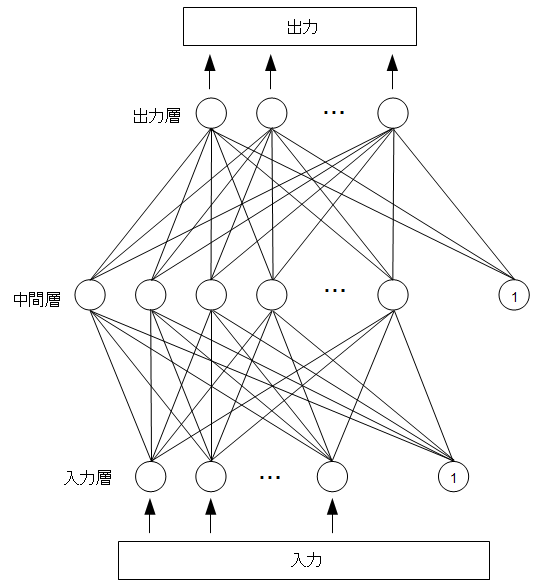
\includegraphics[width=0.45\hsize]{image201003/neuralnet01.png}
\end{center}
\end{figure}

$B$=$l$>$l$N=E$_$O<B?t$GI=$5$l!"%Q!<%;%W%H%m%s$,5!G=$9$k$?$a$K$O$3(B
$B$N=E$_$,E,@Z$K@_Dj$5$l$F$$$kI,MW$,$"$j$^$9!#$"$kF~NO$,M?$($i$l$?(B
$B:]!"F~NOCM$K=E$_$r3]$19g$o$;!"$=$l$>$l$N9g7W$K<!$N$h$&$J%7%0%b%$(B
$B%I4X?t$rE,MQ$7$??tCM$rCf4VAX$N;}$DCM$H$7$^$9!#(B

\begin{multicols}{2}

\begin{figure}[H]
\begin{center}
\caption{$B%7%0%b%$%I4X?t$N<0(B}
\begin{equation*}
 \varsigma_1(x) = \frac{1}{1+e^{-x}}
\end{equation*}
\end{center}
\end{figure}

\begin{figure}[H]
\begin{center}
\caption{$B%7%0%b%$%I4X?t$N%0%i%U(B}
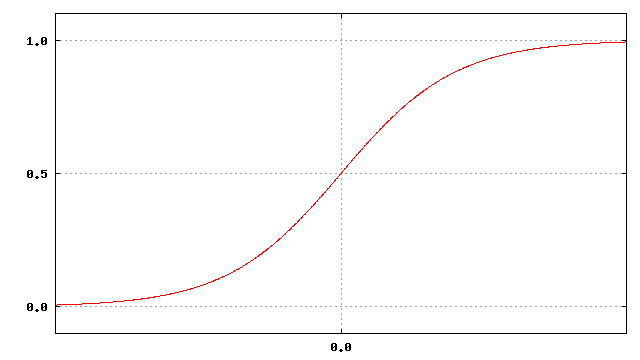
\includegraphics[width=1.0\hsize]{image201003/neuralnet03.png}
\end{center}
\end{figure}

\end{multicols}

$B3F=PNOAX$bF1MM$N7W;;$,$J$5$l!"%Q!<%;%W%H%m%s$N=PNO$,9T$o$l$^$9!#(B

\subsubsection{$B%P%C%/%W%m%Q%2!<%7%g%s(B}

$BB?AX%Q!<%;%W%H%m%s$GE,@Z$J=PNO$r9T$&$?$a$N3X=,J}K!$H$7$F0lHLE*$J(B
$B$b$N$K%P%C%/%W%m%Q%2!<%7%g%s$,$"$j$^$9!#%P%C%/%W%m%Q%2!<%7%g%s$G(B
$B$O$^$:F~NO$KBP$9$k@5$7$$=PNO(B($B65;U?.9f(B)$B$rB??tMQ0U$7!"3F=E$_$r%i%s(B
$B%@%`$K@_Dj$7$^$9!#MQ0U$5$l$?F~NO$KBP$7$F%i%s%@%`$J=E$_$+$i%Q!<%;(B
$B%W%H%m%s$N=PNO$O$G$?$i$a$JCM$H$J$j$^$9$,!"$3$N=PNO$H65;U?.9f$H$N(B
$BHf3S$+$i=PNOAX$HCf4VAX$N4V$N=E$_$r=$@5$7!"<!$$$GCf4VAX$HF~NOAX$N(B
$B=E$_$r=$@5$9$k$3$H$GE,@Z$J=E$_$rC5$7=P$7$^$9!#(B

\subsection{$BB-$7;;$H0z$-;;$r3X=,$7$F$_$k(B}

$B:n@.$7$?%Q!<%;%W%H%m%s$H%P%C%/%W%m%Q%2!<%7%g%s$,@5>o$KF0:n$9$k$+(B
$B$r3N$+$a$^$9!#<!$N$h$&$JF~NO$rMQ0U$7$^$7$?!#(B

\begin{commandline}
# $B3X=,MQ65;U?.9f%Z%"(B
0.40,0.20	0.60,0.20
0.30,0.20	0.50,0.10
0.80,0.10	0.90,0.70
0.20,0.10	0.30,0.10
0.50,0.50	1.00,0.00
0.60,0.20	0.80,0.40
# $BI>2AMQF~NOCM(B
*0.50,0.10
*0.50,0.40
*0.10,0.40
\end{commandline}

$BF~NOCM$H65;U?.9f$N%Z%"$O%?%V6h@Z$j$N:8$,F~NO!"(B
$B1&$,F~NO$KBP$9$k65;U?.9f$G$9!#(B
$B$3$3$G$OB-$7;;$H0z$-;;$N65;U?.9f$rM?$($^$7$?!#(B

\newpage

$B<B9T$7$^$9!#(B

\begin{commandline}
$ ./backprop.exe sample.txt 10000
       0 0.87640153
     100 0.26410368
     200 0.10289131
     300 0.03820243
     400 0.02475167

...($BCfN,(B)...

    9600 0.00077714
    9700 0.00077174
    9800 0.00076646
    9900 0.00076128
0.4000, 0.2000  0.60, 0.18      0.60, 0.20
0.3000, 0.2000  0.50, 0.11      0.50, 0.10
0.8000, 0.1000  0.90, 0.70      0.90, 0.70
0.2000, 0.1000  0.30, 0.11      0.30, 0.10
0.5000, 0.5000  0.98, 0.02      1.00, 0.00
0.6000, 0.2000  0.80, 0.41      0.80, 0.40
0.5000, 0.1000  0.63, 0.35
0.5000, 0.4000  0.93, 0.06
0.1000, 0.4000  0.87, 0.00
Ratio=0.00075626
Count=10000
Sample=6
Input=2
Middle=4
Output=2
InputHidden0=-2.57936471,-2.20525001,-1.50656422,4.05055823,-0.66468037
InputHidden1=-1.29032439,8.71632107,-1.24344376,-0.85214732,-0.66468037
InputHidden2=2.04901840,-2.94096519,1.04866634,-1.98825291,0.29698485
HiddenOutput0=-2.91458436,-1.16992032
HiddenOutput1=5.84673832,-6.31188860
HiddenOutput2=-1.80018561,-0.42470539
HiddenOutput3=3.60356071,3.84028669
HiddenOutput4=1.40998866,-1.22885398
\end{commandline}

$BMj$j$J$$$J$,$i$b$=$l$J$j$N1i;;7k2L$,=PNO$5$l$F$$$^$9!#I>2A$H$7$F(B
$B:G8e$N?tCM$O8:;;7k2L$,Ii$K$J$k$O$:$J$N$G$9$,!"%7%0%b%$%I4X?t$rDL(B
$B$9$3$H$G=PNO$,(B0.0$B!A(B1.0$B$H$J$k$?$a@5>o$J7k2L$,F@$i$l$^$;$s!#(B

\subsection{$B2hA|$rJ,N`$9$k$?$a$NF~NOCM$r9M$($k(B}

$B2hA|H=JL$NF~NOCM$H$7$F<!$NCM$r;HMQ$7$^$7$?!#(B

\begin{itemize}
\item $BJd@5$7$?2hA|$N(BRGB$B$N:9(B
\item $BHyJ,$7$?2hA|$N(BRGB$B$N:9(B
\item $B2hA|$NJ#;($5!#(B
\item $B;H$o$l$F$$$k?'$N?t(B
\item $BJ?6Q:LEY(B
\item FFT$B=hM}$7$?2hA|$NL@$k$$%T%/%;%k$rMxMQ$9$k(B
\item HSV$B$KJQ49$7!"?'AG$NJ?6Q$rMxMQ$9$k(B
\item $B?'AG$NJ,;6$rMxMQ$9$k(B
\end{itemize}

$B$3$NCf$+$iJ8>O$H3($NH=JL$H$7$F2hA|$N(BFFT$B$r!"%+%i!<2hA|$NH=JL$H$7(B
$B$F(BHSV$B$X$NJQ49$r2r@b$7$^$9!#(B

\newpage

\subsubsection{$B%b%N%/%m2hA|$N=hM}!&J8;z$H3($rJ,N`$7$F$_$k(B}

$B=D=q$-$NJ8>O$O2#J}8~$K0lDj$N<~GH?t$r;}$C$F$$$k$H8+$J$9$3$H$,=PMh(B
$B$^$9!#$3$l$K$h$j!"J8>O$N2hA|$rHyJ,$7(BFFT$B=hM}$r9T$C$?7k2L$+$i?6I}(B
$B$rIA2h$9$k$H$G!"L@$k$/8w$kE@$,8=$l$k$3$H$,$o$+$j$^$7$?!#(B

\begin{figure}[H]
\begin{center}
\caption{$B%$%i%9%H$HJ8>O$rHyJ,$7$?2hA|$N(BFFT$B7k2L(B}
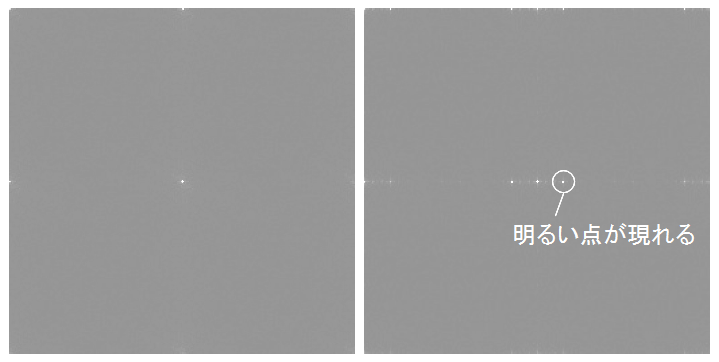
\includegraphics[width=0.9\hsize]{image201003/neuralnet04.png}
\end{center}
\end{figure}

$B$3$NE@$NL@$k$5$rF~NOCM$H$9$k$3$H$G!"J8>O$H%$%i%9%H$NH=JL$,9T$($k(B
$B$H4|BT$G$-$^$9!#(B

\subsubsection{$B%+%i!<2hA|$H$=$&$G$J$$2hA|$rJ,N`$7$F$_$k(B}

$B%+%i!<2hA|$H%b%N%/%m2hA|$O2hA|$N(BRGB$B$r(BHSV$B$KJQ49$7!"?'Aj$+$iH=JL$r(B
$B9T$C$F$$$^$9!#(B

RGB$B$N$&$A$+$i:GBg$N$b$N$r(BMAX$B!":G>.$N$b$N$r(BMIN$B$H$9$k$H?'Aj$O<!$N(B
$B<0$H$J$j$^$9!#(B

\begin{figure}[H]
\begin{center}
\caption{$B?'Aj$N7W;;<0(B}

\begin{align*}
 H = & 60 \frac{G-B}{MAX-MIN} + 0, & if MAX = R\\
     & 60 \frac{B-R}{MAX-MIN} + 120,   & if MAX = G\\
     & 60 \frac{R-G}{MAX-MIN} + 240,   & if MAX = B\\
\end{align*}
\end{center}
\end{figure}

$B%b%N%/%m2hA|$O?'Aj$r;}$?$J$$$?$a!"(BRGB$B$N$&$A@D$N@.J,$r8:$i$9$3$H(B
$B$G2+?'$$%U%#%k%?$r$+$1$^$7$?!#$3$&$9$k$3$H$G%b%N%/%m2hA|$N?'Aj$N(B
$BJ?6Q$O2+?'$H$J$j!"%+%i!<$H%b%N%/%m$rH=JL$9$k$?$a$NF~NOCM$H$7$F4|(B
$BBT$G$-$^$9!#(B

\newpage

\subsection{$B3X=,$N>r7o(B}

$B%K%e!<%i%k%M%C%H$N3X=,$O<!$N>r7o$G9T$$$^$7$?!#(B

\begin{itemize}
\item $BF~NOAX(B8$B8D(B
\item $BCf4VAX(B24$B8D(B
\item $B=PNOAX(B2$B8D(B
\item $B%5%s%W%k$H$7$F;HMQ$7$?K\(B23$B:}(B($BL!2h(B2$B:}(B/$BJ88K(B20$B:}(B/$B5;=Q=q(B1$B:}(B)
\item $B%Z!<%8?t(B6742$B%Z!<%8(B
\item $B3X=,2s?t(B50$BK|2s(B
\end{itemize}

$B<B:]$K$3$N>r7o$G3X=,$r9T$C$?:]!"(B
Core i7 950$B$G(B7$B;~4V<e$N3X=,;~4V$H$J$j$^$7$?!#(B

\subsection{$BH=JL$N@:EY(B}

$B:n@.$5$l$?%D!<%k$G<B:]$KH=JL$r9T$$!"$=$N@:EY$rD4$Y$^$7$?!#I>2A$K(B
$B;HMQ$7$?K\$O3X=,$K;H$o$l$F$$$J$$$b$N$rA*$S$^$7$?!#(B

\begin{description}
 \item[$B%5%s%W%k(B1. $B%i%$%H%N%Y%k:G?74,(B] \mbox{}\\
    240$B%Z!<%8Cf!"?M4V$NH=JL$H?)$$0c$&%Z!<%8$,(B2$B%Z!<%8!#FbLu$O%+%i!<(B
    12$B%Z!<%8!"%0%l!<%9%1!<%k(B15$B%Z!<%8!"J8>O(B213$B%Z!<%8!#$=$N$&$A%$(B
    $B%i%9%H$,J8>O$HH=JL$5$l$?$N$,(B1$B%Z!<%8!"J8>O$,%$%i%9%H$HH=JL$5(B
    $B$l$?$N$,(B1$B%Z!<%8!#(B
 \item[$B%5%s%W%k(B2. SF$BD9JT%7%j!<%:$N>e4,(B] \mbox{}\\
    568$B%Z!<%8Cf!"?M4V$NH=JL$H?)$$0c$&%Z!<%8$O$J$7!#FbLu$O%+%i!<(B5
    $B%Z!<%8!"%0%l!<%9%1!<%k(B3$B%Z!<%8!"J8>O(B560$B%Z!<%8!#(B
 \item[$B%5%s%W%k(B3. $B%m!<%^?M$N%7%j!<%:(B1$B4,(B] \mbox{}\\
    216$B%Z!<%8Cf!"?M4V$NH=JL$H?)$$0c$&%Z!<%8$O(B5$B%Z!<%8!#FbLu$O%+%i!<(B
    6$B%Z!<%8!"%0%l!<%9%1!<%k(B9$B%Z!<%8!"J8>O(B201$B%Z!<%8!#$=$N$&$A%+%i!<(B
    4$B%Z!<%8$NH=JL$K<:GT$7$F$$$^$9$,!"860x$O%+%P!<%Z!<%8$,%Y!<%8%e(B
    $B$GJ8>O$H$7$FH=JL$5$l$^$7$?!#CO?^$d%$%i%9%H$HJ8>O$,:.$8$C$?%Z!<(B
    $B%8$b3X=,DL$jJ8>O$H$7$FH=JL$5$l$F$$$^$9!#(B
 \item[$B%5%s%W%k(B4. 50$BG/A0$KH/9T$5$l$?3)@n>^<u>^:n(B] \mbox{}\\
    40$BG/6a$/A0$K=PHG$5$l$?K\$G!"(B280$B%Z!<%8Cf!"?M4V$NH=JL$H?)$$0c(B
    $B$&%Z!<%8$,(B16$B%Z!<%8!#FbLu$O%+%i!<(B6$B%Z!<%8!"J8>O(B274$B%Z!<%8!#H=JL(B
    $B$N<:GT$,B?$$M}M3$OJQ?'$H?dB,$5$l!"%+%i!<$@$1$G$O$J$/%$%i%9%H(B
    $B$H$bB?$/4V0c$C$FH=JL$5$l$^$7$?!#(B
\end{description}

%-------------------------------------------------------------------------------
\dancersection{Weka$B$r;H$C$F$_$k(B}{$BA0ED9LJ?(B}
%-------------------------------------------------------------------------------
\index{Weka}
\subsection{$B35MW(B}

$B%K%e!<%i%k%M%C%H%o!<%/$r$O$8$a$H$9$k%G!<%?%^%$%K%s%0$r0lHL?M$,;H$&$K$O!"(B
$BK\>1$5$s$N%M%?$N$h$&$KM}O@$rM}2r$7$?>e$G<+J,$G%W%m%0%i%`$r:n$i$J$$$H$$$1(B
$B$J$$$H$9$k$H!"Hs>o$K%O!<%I%k$,9b$$$H;W$$$^$9!#3X@8$N$3$m$K3X$s$@$j!"8&5f(B
$B$7$F$$$?$+!";E;v$H$7$FIaCJ$+$i07$C$F$$$k$h$&$J?M$G$J$1$l$P!"C18l$H$7$F$O(B
$B<*$K$7$?$3$H$,$"$C$F$b!"$J$s$@$+$h$&J,$+$i$s!"$H$$$&?M$,$[$H$s$I$G$O$J$$(B
$B$G$7$g$&$+!#(B\footnote{Debian $BJY6/2q$N>oO"$O$`$7$mCN$C$F$$$k?M$NJ}$,B?$$(B
$B$N$+$b$7$l$^$;$s$,!">/$J$/$H$b;d$OC18l$r<*$K$7$?$3$H$,$"$k%l%Y%k$G$9!#(B}

$B$=$3$G!"%P%C%/%0%i%&%s%I$H$7$F%K%e!<%i%k%M%C%H%o!<%/$@$1$G$J$/!"%G!<%?%^(B
$B%$%K%s%0$N4pACCN<1$r;}$C$F$$$J$$;d$HF1$8$h$&$JN)>l$N?M$G$b!"(BDebian $B$J$i(B
$B5$7Z$K;n$7$F$_$k4D6-$r@0$($F!"<h$j9g$($:;H$C$F$_$k$3$H$,$G$-$k$h!"$H$$$&(B
$B<q;]$G!"(BWeka $B$H$$$&%D!<%k$r>R2p$7$^$9!#(B

\subsection{Weka$B$H$O(B}

Weka $B$H$O!"(B``Waikato Environment for Knowledge Analysis''$B$NN,$G!"%K%e!<(B
$B%8!<%i%s%I$N9qN)%o%$%+%HBg3X(B\footnote{\url{http://www.waikato.ac.nz/}}$B$G(B
GPL $B$N$b$H%*!<%W%s%=!<%9$G3+H/$5$l$F$$$k%G!<%?%^%$%K%s%0%D!<%k$G$9!#(B
\footnote{\url{http://www.cs.waikato.ac.nz/~ml/weka/index.html}} Java $B$G(B
$B=q$+$l$F$$$^$9!#(B

\subsection{$B%$%s%9%H!<%k(B}

Debian $B$G$O%Q%C%1!<%8$,MQ0U$5$l$F$$$^$9!#(B

\begin{commandline}
$ sudo apt-get install weka
\end{commandline}

\subsection{Weka$B$N;H$$J}(B}

$B%3%^%s%I%i%$%s$G(B \texttt{weka} $B%9%/%j%W%H$r<B9T$7$^$9!#(B

\begin{commandline}
$ weka &
\end{commandline}

$B$9$k$H(B Weka $B$N%&%#%s%I%&$,5/F0$7$^$9!#(B

\begin{figure}[H]
\begin{center}
\caption{Weka $B5/F0%a%K%e!<(B}
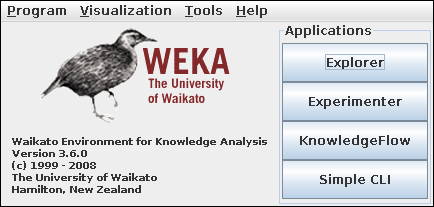
\includegraphics[width=0.5\hsize]{image201003/weka0.png}
\end{center}
\end{figure}

``Applications'' $B$N(B ``Explorer''$B$r<B9T$7$^$9!#(B

\begin{figure}[H]
\begin{center}
\caption{Weka Explorer}
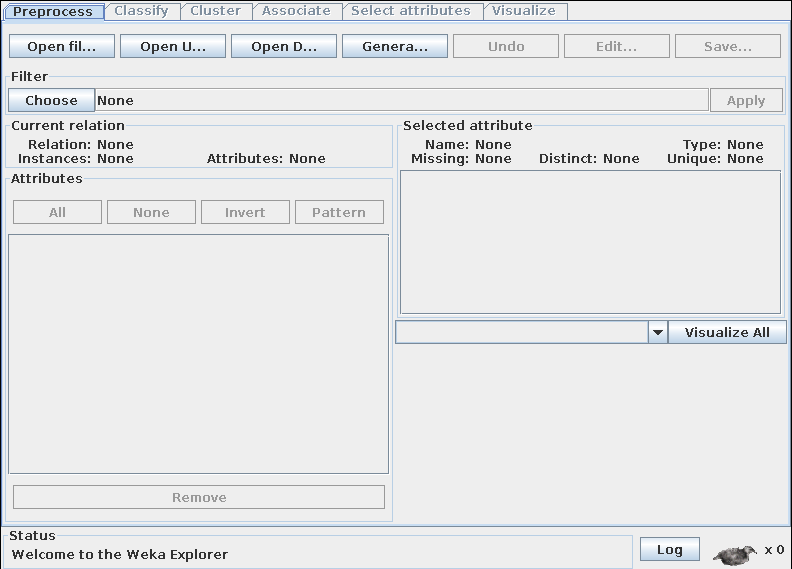
\includegraphics[width=1.0\hsize]{image201003/weka1.png}
\end{center}
\end{figure}

Weka Explorer $B$,5/F0$7$^$9!#(B


\hrule
{\LARGE $B%3%i%`(B: $BB>$N(B OS $B>e$G$N<B9T(B}

Debian $B$G$O%Q%C%1!<%8$,MQ0U$5$l$F$$$^$9$,!"3+H/85$N%5%$%H$G$OB>$N4D6-8~(B
$B$1$N%P%$%J%j%Q%C%1!<%8$,MF0W$5$l$F$$$^$9!#(B
\footnote{\url{http://www.cs.waikato.ac.nz/~ml/weka/index.html}} $B%P%$%J(B
$B%j%Q%C%1!<%8$,MF0W$5$l$F$$$J$/$F$b!"(Bweka.jar $B$,3JG<$5$l$?(B ZIP $B%"!<%+%$%V(B
$B$bMQ0U$5$l$F$$$k$N$G!"(BJava $B%i%s%?%$%`$,$"$k$J$i2<5-$N$h$&$K<B9T$9$l$P(B Debian $B>e$HF1$8$h$&$K;H$&$3$H$,$G$-$^$9!#(B

\begin{commandline}
$ java -jar weka.jar
\end{commandline}

\hrule

\subsubsection{Weka $B$G07$&%G!<%?%U%)!<%^%C%H(B}

Weka $B$G$O!"(BARFF(Attribute-Relation File Format)$B$H$$$&%U%)!<%^%C%H$N%F%-(B
$B%9%H%U%!%$%k$rF~NO%G!<%?$H$7$F07$$$^$9!#(B

$B%G!<%?%U%)!<%^%C%H$O<!$N$h$&$K$J$j$^$9!#(B

\begin{commandline}
@relation $BL>A0(B
@attribute $BB0@-L>(B $BB0@-$N7?(B
@attribute $BB0@-L>(B $BB0@-$N7?(B
:
:
@data
$B%G!<%?(B,$B%G!<%?(B,$B!D(B,$B%G!<%?(B
\end{commandline}

\begin{itemize}
\item @relation $B$O%G!<%?A4BN$NL>A0$r;XDj$7$^$9!#(B
\item @attribute $B$O%G!<%?$NB0@-$rI=$7!"(B1$B$DL\$N0z?t$OB0@-L>!"(B2$B$D$a$N0z?t(B
      $B$OB0@-%G!<%?$N7?$rI=$7$^$9!#(B
\item @attribute $B$N%G!<%?7?$K$O!"(Bnumeric, real, integer, string, date$B7?(B
      $B$r;H$($^$9!#(B
      \begin{itemize}
       \item numeric $B$O(B real $B$+(B integer $B$r;XDj$G$-$^$9!#(B
       \item real $B$O<B?t$r;XDj$G$-$^$9!#(B
       \item integer $B$O@0?t$r;XDj$G$-$^$9!#(B
       \item string $B$OJ8;zNs$r;XDj$G$-$^$9!#(B
       \item date $B7?$OF|;~$G!"%G%U%)%k%H$O(B''yyyy-MM-dd'T'HH:mm:ss''$B$H$$(B
	     $B$&=q<0$G$9!#(B
      \end{itemize}
 \item @data $B%G!<%?NN0h$N@k8@$G$9!#(B
       \begin{itemize}
	\item $B$=$N<!$N9T$+$i(B CSV $B7A<0$G%G!<%?$r5-=R$7$^$9!#(B
	\item @attribute $B9T$G>e$+$i@_Dj$7$?=g$K(B CSV $B$N0l9T$G$N:8$+$i1&$X(B
	      $B$N3F%G!<%?$H$J$j$^$9!#(B
       \end{itemize}
\end{itemize}

$B:rG/$N(B11$B7n$NJY6/2q$G(B GNU R $B$G07$C$?8wG.Hq$N%G!<%?$H!"5$>]D#$,8x3+$7$F$$(B
$B$k5$29!"9_?eNL$J$I$N5$>]%G!<%?(B\footnote{\url{http://www.data.jma.go.jp/obd/stats/etrn/index.php}}$B$r;H$C$F$_$^$9!#(B

$B$^$:!"(BCSV $B$G0J2<$N$h$&$K5-=R$7$?$H$7$^$9!#(B
\begin{commandline}
"$BG/(B","$B7n(B","$B9_?eNL9g7W(B(mm)","$BJ?6QF|J?6Q5$29(B($B!n(B)","$BJ?6QF|:G9b5$29(B($B!n(B)","$BJ?6QF|:GDc5$(B
$B29(B($B!n(B)","$BJ?6QIwB.(B(m/s)","$B:GBgIwB.(B(m/s)","$BF|>H;~4V(B(h)","$BEE5$;HMQNL(B(kWh)","$BEE5$;HMQ(B
$BNL(B(kWh)/$BF|(B","$BNA6b(B($B1_(B)/$BF|(B","$B9g7WNA6b(B","$B%,%9;HMQNL(B(m3)","$B%,%9;HMQNL(B(m3)/$BF|(B","$BNA6b(B(
$B1_(B)/$BF|(B","$B9g7WNA6b(B"
2007,1,50,6,10.8,1.1,1,5,188.9,234,6.88235294117647,161.235294117647,5482,9,0.257142857142857,70.1714285714286,2456
2007,2,44,7.3,12.6,1.9,1.3,6,198.1,198,7.07142857142857,168.071428571429,4706,9,0.333333333333333,80.962962962963,2186
(snip)
\end{commandline}

$B$3$l$O!"(BARFF $B%U%)!<%^%C%H$G$O0J2<$N$h$&$K$J$j$^$9!#(B

\begin{commandline}
@relation $B9_?eNL!&5$29(B($BI\Cf;T(B)$B$HEE5$Be!"%,%9Be$N4X78$K$D$$$F(B

@attribute $BG/(B real
@attribute $B7n(B real
@attribute $B9_?eNL9g7W(B(mm) real
@attribute $BJ?6QF|J?6Q5$29(B($B!n(B) real
@attribute $BJ?6QF|:G9b5$29(B($B!n(B) real
@attribute $BJ?6QF|:GDc5$29(B($B!n(B) real
@attribute $BJ?6QIwB.(B(m/s) real
@attribute $B:GBgIwB.(B(m/s) real
@attribute $BF|>H;~4V(B(h) real
@attribute $BEE5$;HMQNL(B(kWh) real
@attribute $BEE5$;HMQNL(B(kWh)/$BF|(B real
@attribute $BNA6b(B($B1_(B)/$BF|(B real
@attribute $B9g7WNA6b(B real
@attribute $B%,%9;HMQNL(B(m3) real
@attribute $B%,%9;HMQNL(B(m3)/$BF|(B real
@attribute $BNA6b(B($B1_(B)/$BF|(B real
@attribute $B9g7WNA6b(B real

@data
2007,1,50,6,10.8,1.1,1,5,188.9,234,6.88235294117647,161.235294117647,5482,9,0.257142857142857,70.1714285714286,2456
2007,2,44,7.3,12.6,1.9,1.3,6,198.1,198,7.07142857142857,168.071428571429,4706,9,0.333333333333333,80.962962962963,2186
(snip)
\end{commandline}

\subsubsection{ARFF $B$r%m!<%I$9$k(B}

$B@h$[$IMQ0U$7$?(B kohnetsu.arff $B$r%m!<%I$7$F$_$^$7$g$&!#(BPreprocess $B%?%V$N(B
Open File $B%\%?%s$r2!$7$^$9!#%@%$%"%m%0$,I=<($5$l$k$N$G!"(Bkohnetsu.arff $B$r(B
$B;XDj$7$^$9!#(B

\begin{figure}[H]
\begin{center}
\caption{ARFF $B%U%!%$%k$r%m!<%I$9$k(B}
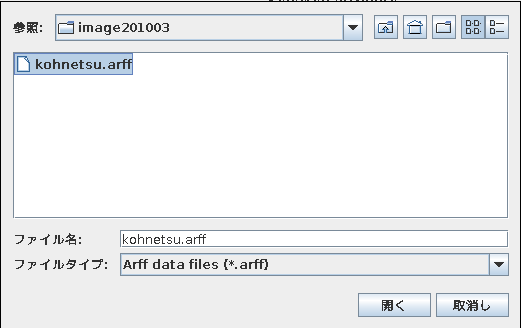
\includegraphics[width=0.5\hsize]{image201003/weka2.png}
\end{center}
\end{figure}

ARFF $B%U%!%$%k$rFI$_9~$`$H0J2<$N$h$&$K$J$j$^$9!#(BUTF-8 $B%(%s%3!<%I$G$"$l$P!"(B
$B$4Mw$N$H$*$jF|K\8l$b@5>o$KFI$_9~$a$^$9(B

\begin{figure}[H]
\begin{center}
\caption{ARFF $B$+$i%G!<%?$rFI$_9~$s$@7k2L(B}
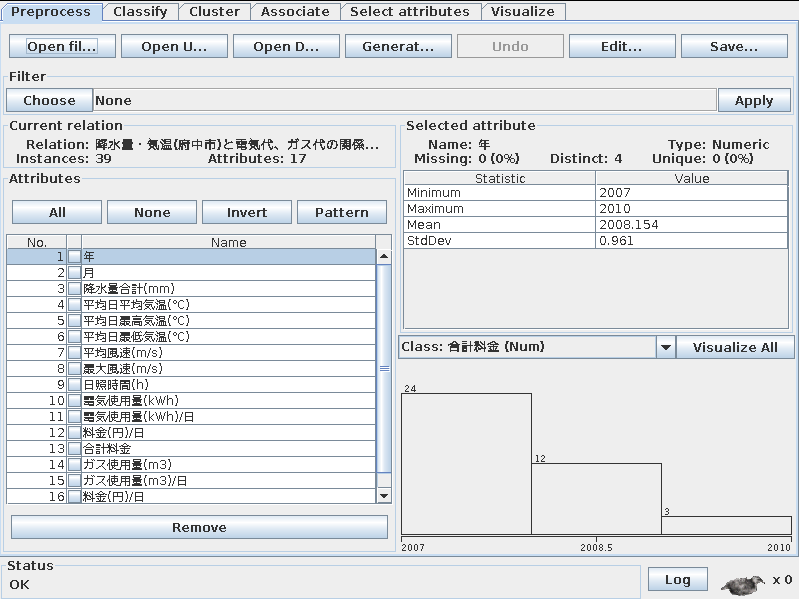
\includegraphics[width=1.0\hsize]{image201003/weka3.png}
\end{center}
\end{figure}

\subsubsection{$B2D;k2=$7$F$_$k(B}

$B$=$l$G$OFI$_9~$s$@%G!<%?$r2D;k2=$7$F$_$^$7$g$&!#(BVisualize $B%?%V$r%/%j%C%/(B
$B$9$k$H<!$N$h$&$J%^%H%j%C%/%9$,I=<($5$l$^$9!#(B

\begin{figure}[H]
\begin{center}
\caption{Visualize $B2hLL(B}
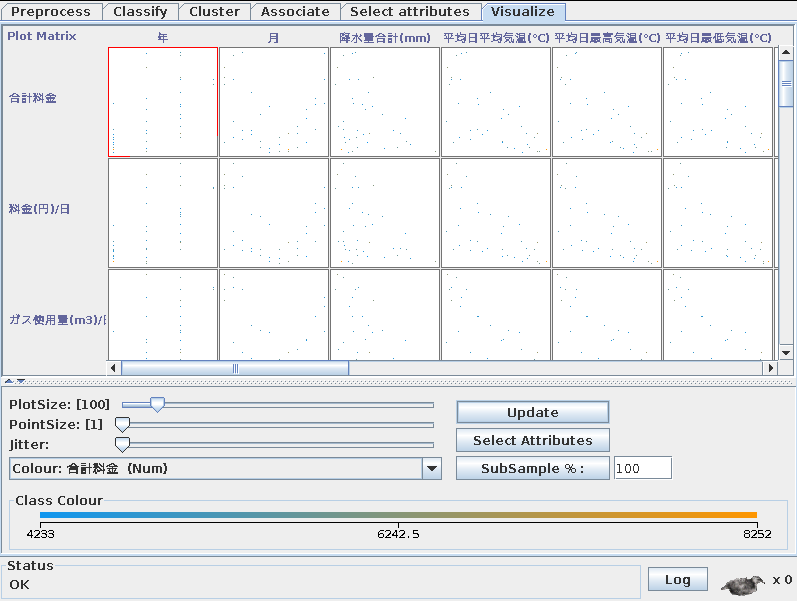
\includegraphics[width=1.0\hsize]{image201003/weka4.png}
\end{center}
\end{figure}

$BE,Ev$K3+$$$F$_$^$9!#(BY $B<4$K0lF|$NJ?6Q5$29$N7nJ?6Q(B($B!n(B)$B$H!"(B X $B<4$K0lF|$"$?(B
$B$j$NEE5$;HMQNL(B(kWh)$B$r<h$C$F8+$F$_$k$H<!$N$h$&$K$J$j$^$9!#(B

\begin{figure}[H]
\begin{center}
\caption{Visualize $B>\:Y2hLL(B}
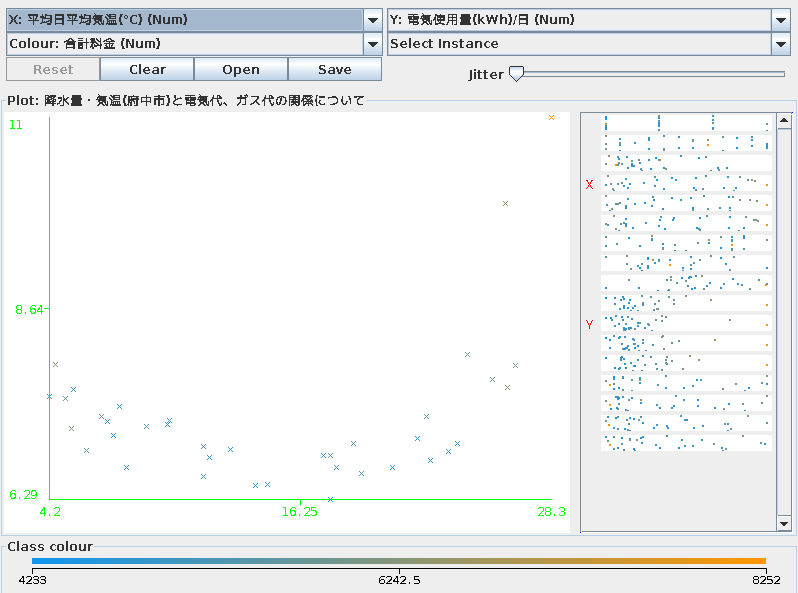
\includegraphics[width=1.0\hsize]{image201003/weka5.png}
\end{center}
\end{figure}


\subsubsection{$BJ,N`$7$F$_$k(B}

$B<!$KJ,N`$7$F$_$^$9!#(BClassify $B%?%V(B $B"*(B Choose $B%\%?%s$r2!$7!"I=<($5$l$?%D%j!<(B
$B$+$i(BMultilayer Perceptron ($B%K%e!<%i%k%M%C%H%o!<%/$K$h$kJ,N`(B)$B$rA*Br$7$^$9!#(B
$B<!$K!"(B(Num)$BJ?6QF|J?6Q5$29(B($B!n(B) $B$rL\E*4X?t$H$7$FA*Br$7$^$9!#(B

\begin{figure}[H]
\begin{center}
\caption{Classify $B2hLL(B}
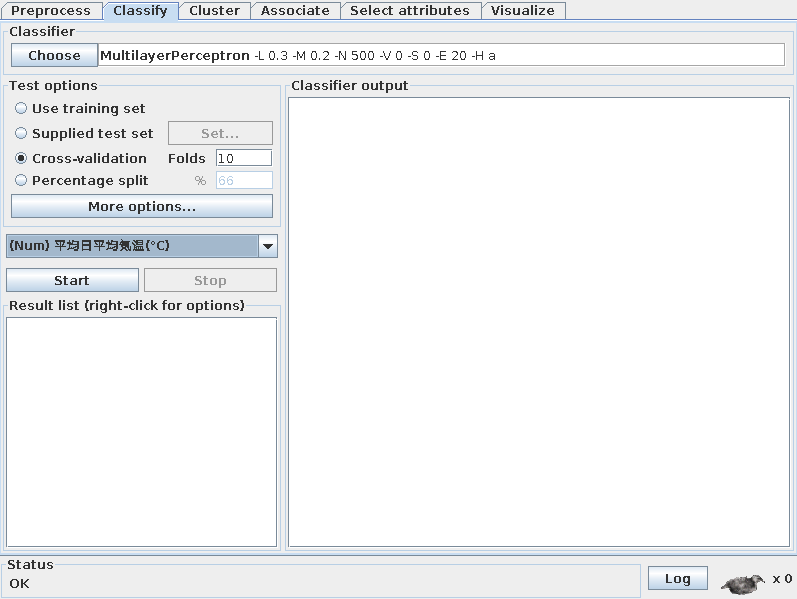
\includegraphics[width=1.0\hsize]{image201003/weka6.png}
\end{center}
\end{figure}

Start $B%\%?%s$r%/%j%C%/$9$k$HJ,N`$,<B9T$5$l!"7k2L$,I=<($5$l$^$9!#(B

\begin{figure}[H]
\begin{center}
\caption{Classify $B7k2L(B}
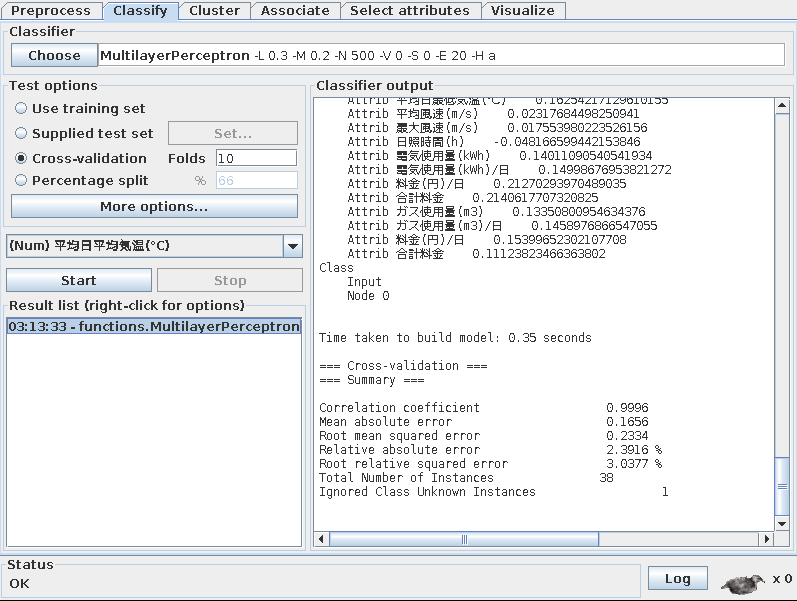
\includegraphics[width=1.0\hsize]{image201003/weka7.png}
\end{center}
\end{figure}

\subsection{$B;29MJ88%(B}
\begin{itemize}
 \item \url{www1.doshisha.ac.jp/~mjin/R/23.pdf}
 \item \url{http://web.sfc.keio.ac.jp/~soh/dm03/man_w_03.html}
 \item \url{http://weka.wikispaces.com/ARFF}
\end{itemize}

%-------------------------------------------------------------------------------
\dancersection{man-db $B$r?<DI$$$7$?(B}{$BF|HfLn(B $B7<(B}
%-------------------------------------------------------------------------------
\index{man-db}
\index{groff}

\subsection{$BF|K\8l$N(Bman$B$,JQ(B}

$B$3$s$J46$8(B

\par
\includegraphics[width=120mm]{image201003/manls.eps}

$BF|K\8l$NJ8;z$NI=<(I}$,%"%k%U%!%Y%C%H$HF1$8$@$HH=Dj$5$l$F$7$^$C$F$$$k$N$G!"(B
$B7k2LE*$KF|K\8l$G=q$+$l$?9T$ND9$5$,G\$0$i$$$K$J$C$F$7$^$C$F$$$^$9!#(B

\subsection{$B2r$O(Bgroff$B$K$"$j(B}

\subsubsection{$B$=$b$=$b(Broff$B$C$F$I$&$$$&$b$N(B?}

$B$H$F$bC1=c$K8@$($P!"%?%$%W%i%$%?!<$_$?$$$J$b$N$G$9!#(B


\subsubsection{roff$BJ8;zI}$N;XDj(B}

$B0JA0$N%P!<%8%g%s$N(Bgroff$B$G$OF|K\8l$NJ8;z$NI=<(I}$,%"%k%U%!%Y%C%H$NG\$G$"$k$3$H$r(B
unicode$B$N(Bcode point$B$NHO0O$G@_Dj$7$F$"$j$^$7$?!#(B
$BF|K\8l$NJ8;z(B


$B2r7h0F(B($B8=;~E@$G$NA[A|(B)$B$r7G:\!#(B

$B%5%9%Z%s%9$b$N!#(B

%-------------------------------------------------------------------------------
\dancersection{Debian $B$G(B libfftw $B$r;H$C$F$_$k(B}{$B>e@n=c0l(B}
%-------------------------------------------------------------------------------
\index{fftw}
\index{FFT}
\index{DFT}
\index{libfftw}
\index{libsndfile}

\subsection{$B$O$8$a$K(B}

Debian$B$G(BFFT$B$r<h$j07$&(BC$B$N%"%W%j%1!<%7%g%s$r=q$$$F$_$?$$$H;W$&$3$H$O$"$j(B
$B$^$;$s$+(B?$B:#F|$O2;@<%G!<%?$rJ,@O$7$F$_$^$7$g$&!#(B

wav $B%U%!%$%k$rF~NO$H$7$F<u$1<h$j!"(BFFT$B$r<B9T$7$F$=$N7k2L$rI=<($9$k%"%W%j%1!<(B
$B%7%g%s$r:n@.$7$F$_$^$9!#(B

\subsection{$B%$%s%9%H!<%k(B}

libfftw3 $B$r%$%s%9%H!<%k$7$^$9!#(B
$B$"$H!"2;@<%U%!%$%k$r%m!<%I$9$k$?$a$K(B sndfile1 $B$rMxMQ$7$^$9!#(B

\begin{commandline}
$ apt-get install libfftw3-dev libsndfile1-dev
\end{commandline}
%$

\subsection{$B<B83BP>]$N=`Hw(B:$B4JC1$J(Bsine$BGH$r:n@.$9$k(B}

$B$^$:!"%F%9%HMQ$K(BFFT$B$N7k2L$,M=A[$G$-$k%G!<%?$r:n@.$7$F$_$^$9!#(B
$B$3$3$G$O(B 440Hz $B$N$-$l$$$J%5%$%sGH$r:n@.$7$F$$$^$9!#(B

\begin{equation*}
 data(x) = sin (\frac{2 \pi 440 x}{44100} ) 
\footnote{sin $B$O(B radian}
\end{equation*}

\begin{commandline}
/*BINFMTC: -lsndfile -lm

  Create a sine wave at 44.1kHz for 1 second called sine.wav
 */
#include <stdlib.h>
#include <stdio.h>
#include <sndfile.h>
#include <math.h>

int create_sine(const char* filename, int size, double frequency)
{
  SF_INFO sfinfo = {
    .frames = size,
    .samplerate = 44100,
    .channels = 1,
    .format = SF_FORMAT_WAV | SF_FORMAT_PCM_16,
    .sections = 0,
    .seekable = 0
  };
  SNDFILE* s = sf_open(filename, SFM_WRITE, &sfinfo);
  double* data = malloc(sizeof(double) * size);
  int i;

  for (i=0; i < size; ++i)
    {
      data[i] = sin(frequency * 2.0 * M_PI * i / 44100.0);
    }

  sf_writef_double(s, data, size);
  sf_close(s);
  return 0;
}

int main()
{
  return create_sine("sine.wav", 44100, 440.0);
}
\end{commandline}

\subsection{$B<B83BP>]$N=`Hw(B:$BJ#;($JF~NOCMNc$N=`Hw(B}

$B%F%9%HMQ$NF~NOCM$H$7$F!"E,Ev$J(B wav $B%U%!%$%k$rMQ0U$7$^$7$g$&!#(B

$B:#2s$O<j85$G!"(Baeolus $B$H$$$&%*%k%,%s%7%_%e%l!<%?$r5/F0$7!"(B 
jack $B$G@\B3$5$;!"(Becasound $B$r(B jack $BF~NO$K(B
$BBP$7$FBT5!$5$;!"(Bqjackctl $B$G@\B3$5$;$F<}O?$7$^$7$?!#(B

$B$=$l$J$j$KD9$$;~4VO?2;$7$?%G!<%?$+$i(B 16-bit mono $B$N(B PCM $B%G!<%?(B1$BICJ,$r@Z$j(B
$B=P$7$F<B83MQ%G!<%?$r:n@.$7$^$7$?!#(B

\begin{commandline}
$ qjackctl &
$ aeolus &
$ vkeybd &
$ ecasound -i jack -o test.wav
ctrl-C $B$GCfCG(B
$ sweep test.wav # $BE,Ev$KJT=8(B
$ file ra-mono.wav  # $B@Z$j=P$7$?7k2L$r3NG'(B
ra-mono.wav: RIFF (little-endian) data, WAVE audio, Microsoft PCM, 16 bit, mono 44100 Hz
\end{commandline}
%$

\subsection{FFTW$B$r;H$C$F(B wav $B%U%!%$%k$r=hM}$7$F$_$k(B}

sndfile $B$H(B fftw3 $B$r;H$C$F%U!<%j%(JQ49$7$F=PNO$r%@%s%W$7$F$_$^$7$g$&!#%5%s(B
$B%W%k%3!<%I$O(B sndfile $B$r;H$$(B double $B$NG[Ns$K(Bwav$B%U%!%$%k$NCf?H$rE83+$7$F!"(B
$B$=$NFbMF$r(B fftw $B$KEO$7$F=hM}$7$F$$$^$9!#(Bdouble $B$NCM$O3F(B 1/44100 $BIC$N=V4V(B
$B$K$*$1$k6u5$$N05NO$rI=$7$F$$$k$h$&$G$9!#(B

\begin{commandline}
/*BINFMTC: -lsndfile -lfftw3 -lm
 */

#include <stdlib.h>
#include <stdio.h>
#include <sndfile.h>
#include <math.h>
#include <complex.h>
#include <fftw3.h>

/*
  process with FFTW
 */
void study_sound(double* data, int size)
{
  fftw_complex* spectrum;
  fftw_plan p;
  int i;

  spectrum = (fftw_complex*) fftw_malloc(sizeof(fftw_complex) * (size / 2 + 1));
  p = fftw_plan_dft_r2c_1d(size, data, spectrum, FFTW_ESTIMATE);

  /* process with FFTW */
  fftw_execute(p);

  /* dump output in CSV format */
  printf("i,abs,arg\n");
  for (i=0; i<(size/2+1); ++i) {
    printf("%i,%f,%f\n", i,
	   cabs(spectrum[i]),
	   carg(spectrum[i]) / 2.0 / M_PI * 360.0);
  }
  fftw_destroy_plan(p);
  fftw_free(spectrum);
}

/*
  Process wav file.

  @return 1 on failure, 0 on success.
*/
int process_wav_file(const char* filename, int size)
{
  SF_INFO sfinfo = {0, 0, 0, 0, 0, 0};
  SNDFILE* s = sf_open(filename, SFM_READ, &sfinfo);
  double* data = malloc(sizeof(double) * size);

  if (!s || !data)
    {
      fprintf(stderr,
	      "Something went wrong opening the file or allocating memory\n");
      return 1;
    }
  if (sfinfo.channels != 1)
    {
      fprintf(stderr,
	      "Please give me monaural audio data\n");
      return 1;
    }

  /* Read wav file into an array of double */
  sf_readf_double(s, data, size / sfinfo.channels);
  study_sound(data, size / sfinfo.channels);
  sf_close(s);
  return 0;
}

int main(int argc, char** argv)
{
  process_wav_file(argv[1], atoi(argv[2]));
  return 0;
}
\end{commandline}

$B<B9T$7$F$_$^$9!#(B

\begin{commandline}
$ ./sndfile-fftw.c sine.wav 44100 > sine.csv
$ ./sndfile-fftw.c ra-1sec.wav 44100 > ra.csv
\end{commandline}
%$

\subsection{$B=PNO$r3NG'$7$F$_$k(B}

CSV$B%U%!%$%k7A<0$G%G!<%?$,=PNO$5$l$^$7$?!#(B
$B4JC1$K%0%i%U$r:n@.$9$k$?$a$N%D!<%k$H$7$F$3$3$G$O(BR$B$r;H$C$F$_$^$9!#(B

\begin{commandline}
$ R

R version 2.7.1 (2008-06-23)
Copyright (C) 2008 The R Foundation for Statistical Computing
ISBN 3-900051-07-0

R$B$O%U%j!<%=%U%H%&%'%"$G$"$j!"!V40A4$KL5J]>Z!W$G$9!#(B 
 $B0lDj$N>r7o$K=>$($P!"<+M3$K$3$l$r:FG[I[$9$k$3$H$,$G$-$^$9!#(B 
$BG[I[>r7o$N>\:Y$K4X$7$F$O!"(B'license()'$B$"$k$$$O(B'licence()'$B$HF~NO$7$F$/$@$5$$!#(B 

R$B$OB?$/$N9W8%<T$K$h$k6&F1%W%m%8%'%/%H$G$9!#(B 
$B>\$7$/$O(B'contributors()'$B$HF~NO$7$F$/$@$5$$!#(B 
$B$^$?!"(BR$B$d(BR$B$N%Q%C%1!<%8$r=PHGJ*$G0zMQ$9$k:]$N7A<0$K$D$$$F$O(B 
'citation()'$B$HF~NO$7$F$/$@$5$$!#(B 
 
'demo()'$B$HF~NO$9$l$P%G%b$r$_$k$3$H$,$G$-$^$9!#(B 
'help()'$B$H$9$l$P%*%s%i%$%s%X%k%W$,=P$^$9!#(B 
'help.start()'$B$G(BHTML$B%V%i%&%6$K$h$k%X%k%W$,$_$i$l$^$9!#(B 
'q()'$B$HF~NO$9$l$P(BR$B$r=*N;$7$^$9!#(B 

> sine <- read.csv("sine.csv")
> ra <- read.csv("ra.csv")
> summary(sine)
       i              abs                 arg           
 Min.   :    0   Min.   :    0.000   Min.   :-179.9674  
 1st Qu.: 5512   1st Qu.:    0.000   1st Qu.:   0.0000  
 Median :11025   Median :    0.000   Median :   0.0000  
 Mean   :11025   Mean   :    1.000   Mean   :  -0.1395  
 3rd Qu.:16538   3rd Qu.:    0.000   3rd Qu.:   0.0000  
 Max.   :22050   Max.   :22049.319   Max.   : 180.0000  
> summary(ra)
       i              abs                 arg         
 Min.   :    0   Min.   :2.066e-03   Min.   :-179.93  
 1st Qu.: 5512   1st Qu.:1.467e-02   1st Qu.: -56.88  
 Median :11025   Median :1.907e-02   Median : -37.80  
 Mean   :11025   Mean   :3.944e-01   Mean   : -38.40  
 3rd Qu.:16538   3rd Qu.:3.620e-02   3rd Qu.: -17.82  
 Max.   :22050   Max.   :4.072e+02   Max.   : 180.00  

> postscript("sine.eps", horizontal=FALSE, height=3, width=3)
> plot(sine$i, sine$abs, xlim=c(400,500), ylim=c(0,22000), type="l")
> dev.off()
> postscript("ra.eps", horizontal=FALSE, height=3, width=3)
> plot(ra$i, ra$abs, xlim=c(0,2000), ylim=c(0,100), type="l")
> dev.off()
\end{commandline}


\fgref{fig:wave-sine}$B$N(B440Hz $B$N%5%$%sGH$r=hM}$7$?7k2L$r8+$F$_$k$H!"(B440
Hz $B$"$?$j$K%0%i%U$NFM5/$,$"$k$N$,8+$F<h$l$^$9!#(B

\begin{figure}[ht]
 \begin{center}
  \includegraphics{image201003/sine.eps}
 \end{center} 
 \label{fig:wave-sine}
 \caption{440Hz $B$N%5%$%sGH(B}
\end{figure}

$B$7$+$7!"<B:]$K%*%k%,%s2;$r=hM}$7$?7k2L$N(B\fgref{fig:wave-ra}$B$r8+$F$_$k$H!"(B
$B%0%i%U$KFM5/$,B??t$"$C$F!"7k9=J#;($G$9!#$=$N$^$^4JC1$K=hM}$5$;$F$/$l$O$7(B
$B$J$5$=$&$G$9!#(B

\begin{figure}[ht]
 \begin{center}
  \includegraphics{image201003/ra.eps}
 \end{center} 
 \label{fig:wave-ra}
 \caption{$B%i$r(Baeolus$B$GE,Ev$K1iAU$7$?2;(B}
\end{figure}

%-------------------------------------------------------------------------------
\dancersection{``3.0 (quilt)''$B$K$D$$$F(B}{$B5HLnM?;V?N(B}
%-------------------------------------------------------------------------------
\subsection{$B$O$8$a$K(B}
$BIaCJ(BDebian$B$r;H$C$F$$$k3'$5$s$O$4B8CN$H$O;W$$$^$9$,!"6a!9%G%U%)%k%H$K$J$k(B
$BM=Dj$G(Bsqueeze$B$N(Brelease goal$B$G$"$k(BDebian$B%=!<%9%Q%C%1!<(B
$B%8$N%U%)!<%^%C%H(B``\verb|3.0 (quilt)|'' $B$NI|=,$r$7$?$$$H;W$$$^$9!#(B
\subsection{``1.0''}
$B$^$:$O(B``\verb|3.0 (quilt)|''$B$NA0$K!"$$$^$^$G0lHL$K;H$o$l$F$-$?%U%)!<%^%C%H(B(``\verb|1.0|'')$B$r4JC1$K$^$H$a$^$9!#(B

\verb|1.0|$B$G$O!"%=!<%9%Q%C%1!<%8$O0J2<$N(B3$B%U%!%$%k$G9=@.$5$l$^$9!#(B
\begin{itemize}
 \item \textit{packagename}\verb|-|\textit{upstreamversion}\verb|.orig.tar.gz|
 \item \textit{packagename}\verb|-|\textit{debianversion}\verb|.diff.gz|
 \item \textit{packagename}\verb|-|\textit{debianversion}\verb|.dsc|
\end{itemize}

$B$J$*!"@53N$K$O(B\verb|1.0|$B$O(B2$B<oN`$"$C$F!">e$NDL>o$N%Q%C%1!<%8$N$[$+$K(B``Debian
native$B$J(B''$B%Q%C%1!<%8$,$"$j$^$9!#(BDebian native $B%Q%C%1!<%8$O<!$N(B2$B%U%!%$%k$G9=@.$5$l$^$9!#(B
\begin{itemize}
 \item \textit{packagename}\verb|-|\textit{version}\verb|.tar.gz|
 \item \textit{packagename}\verb|-|\textit{version}\verb|.dsc|
\end{itemize}

$B$3$3$G!"(B\verb|*.orig.tar.gz|$B$K$O!"DL>o>eN.$N85$N%=!<%9%D%j!<$,4^$^$l$^$9!#(B
\verb|*.diff.gz|$B$K$O!"%=!<%9%Q%C%1!<%8$+$i%Q%C%1!<%8$J$I$r%S%k%I$9$k$N$KI,MW$J%9%/%j(B
$B%W%H$J$I$,F~$C$?(B \verb|debian/| $B%G%#%l%/%H%j$d!">eN.$N%=!<%9$KBP$9$k%Q%C%1!<%8(B
$B%a%s%F%J$NJQ99$,4^$^$l$^$9!#(B

\subsection{$B$7$+$7(B}
$B$H@bL@$7$F$-$^$7$?$,!"$3$N%U%!%$%k9=@.$K$O(B
\begin{enumerate}
 \item $B%"!<%+%$%V$N05=L7A<0$K(B gzip $B$7$+;H$($J$$(B
 \item $BJ#?t$N%"!<%+%$%V$G9=@.$5$l$k>eN.$N%=!<%9$,$=$N$^$^07$($J$$(B
 \item $B%a%s%F%J$,Ev$F$?%=!<%9$X$N%Q%C%A$,A4It$D$J$,$C$F$7$^$C$F$$$k(B
 \item \verb|debian/| $B0J2<$K%P%$%J%j%U%!%$%k$,D>@\CV$1$J$$(B
\end{enumerate}
$B$J$I$NLdBjE@$,$"$j$^$9!#(B

$B$=$3$G!"$5$^$6$^$JJ}K!$,8!F$$5$l$^$7$?!#(B

1$B$O!"$3$l$K$h$j>eN.$,(Bbz2$B$GG[I[$7$F$$$F$b(Bgz$B$K05=L$7D>$5$J$1$l$P$J$i$J$+$C(B
$B$?$j$7$F$$$^$7$?!#(B\verb|*.orig.tar.gz| $B$NCf?H$,>eN.$N%"!<%+%$%V$N<BBN$G$"$k!"(B
$B$H$$$C$?J}K!$J$I$b!J$A$g$C$HL5BL$G$9$,(B...$B!K;H$o$l$F$-$^$7$?!#$3$NJ}K!$O%S%k%I;~$K$=$N(Btarball$B$rE83+$7$F:n6H(B
$B$7$^$9!#(Bcdbs$B$K$O$3$NJ}K!$X$N%5%]!<%H$b$"$j$^$9!#(B

2$B$O(B1$B$HF1MM$NJ}K!$GJ#?t$N(Btarball$B$,F~$C$?(B\verb|*.orig.tar.gz|$B$rMQ0U$7$?$j(B
$B$7$F$$$^$7$?!#(B

3$B$O!"Ev$?$C$F$$$k%Q%C%A$N$=$l$>$l$,(B
$B$I$s$J0U?^$G9T$o$l$?$N$+$,$o$+$i$J$$!"$H$$$&$3$H!"$^$?!"(B\verb|debian/|$B0J2<$N%U%!(B
$B%$%k$b>eN.%=!<%9$X$N%Q%C%A$b0l=o$/$?$K$J$C$F$7$^$C$F$$$k$3$H!"$,LdBj$G$7$?!#$=$3$G!"$^$H$^$C$?0U(B
$BL#$N$"$kC10L$KJ,3d$5$l$?%Q%C%A$r$^$:MQ0U$7$F$*$-!"$=$l$i$r(B
\verb|debian/patches/| $B2<$KG[CV(B
$B$7!"$=$N:Y$+$$%Q%C%A$r%S%k(B
$B%I;~$KEv$F$k(B/$B30$9%U%l!<%`%o!<%/(B
(patch system) $B$,MxMQ$5$l$F$$$^$9!#$3$l$K$O(B dpatch $B$d(B quilt $B$J$I$,$"$j$^(B
$B$9!#$J$*!"$3$N:Y$+$$%Q%C%A$N$=$l$>$l$K$O!"@hF,$K%Q%C%A$N0U?^$r@bL@$9$kJ8(B
$B>O$r5-=R$9$k$3$H$,?d>)$5$l$F$$$^$9(B(\url{http://dep.debian.net/deps/dep3/})$B!#(B

4$B$O!"%P%$%J%j%U%!%$%k$N(Bdiff$B$r<h$m$&$H$7$F$bIaDL$N(Bpatch$B$G$O$G$-$J$$$3$H$,(B
$B860x$J$N$G!"(Buuencode$B$J$I$G%F%-%9%H$KMn$H$7$F(Bpatch$B$r<h$k!"$H$$$C$?<jK!$,(B
$BMQ$$$i$l$F$-$^$7$?!#(B

\subsection{$B$=$3$G(B}
$B$3$N$h$&$JLdBj$r2r7h$9$k$?$a$K?7$?$J%=!<%9%Q%C%1!<%8$N%U%)!<%^%C%H$b8!F$(B
$B$5$l$^$7$?!#$=$l$,(B``\verb|3.0 (quilt)|''$B%U%)!<%^%C%H!J$H(B``\verb|3.0 (native)|''$B%U%)!<%^%C%H!K$G$9!#(B

\verb|3.0 (quilt)|$B$O<!$N(B3$B$D0J>e$N%U%!%$%k$G9=@.$5$l$^$9!#(B
\begin{itemize}
 \item \textit{packagename}\verb|-|\textit{upstreamversion}\verb|.orig.tar.|\textit{ext}
 \item
      \textit{packagename}\verb|-|\textit{upstreamversion}\verb|.orig-|\textit{component}\verb|.tar.|\textit{ext}$B!JG$0U!K(B
 \item \textit{packagename}\verb|-|\textit{debianversion}\verb|.debian.tar.|\textit{ext}
 \item \textit{packagename}\verb|-|\textit{debianversion}\verb|.dsc|
\end{itemize}

$B$J$*!"(B\verb|1.0|$B$K$"$C$?(BDebian native$B%Q%C%1!<%8$KAjEv$9$k(B\verb|3.0 (native)|$B$O(B
$B<!$N(B2$B%U%!%$%k$G9=@.$5$l$^$9!#(B
\begin{itemize}
 \item \textit{packagename}\verb|-|\textit{version}\verb|.tar.|\textit{ext}
 \item \textit{packagename}\verb|-|\textit{version}\verb|.dsc|
\end{itemize}

$B$3$3$G!"$^$:!"(Btar$B$N3HD%;RItJ,(B\textit{ext}$B$K(B gz $B$N$[$+!"(Bbz2, lzma, xz $B$,MxMQ$G$-(B
$B$k$h$&$K$J$j$^$7$?!#$3$l$K$h$jLdBj(B1$B$,2r7h$5$l$^$7$?!J(B\verb|3.0 (native)|$B$K(B
$B$*$1$k<g$JJQ99E@$O$3$l$G$9!K!#(B

$B$^$?!"(B\textit{component}$B$NItJ,$rE,Ev$KJQ$($k$3$H$K$h$jJ#?t$N(Btarball$B$r$-$A(B
$B$s$H07$($k$h$&$K$J$j$^$7$?!#$3$l$,LdBj(B2$B$r2r7h$7$^$9!#(B

$B<!$K!"(B\verb|debian/|$B2<$N%U%!%$%k$O$9$Y$F(B \verb|*.debian.tar.gz| $B$KF~$l$k$3$H$K(B
$B$J$j$^$7$?!#$3$l$G$9$Y$F$,:.$6$C$?>uBV$O$J$/$J$j$^$7$?!#$5$i(B
$B$K!"(B\verb|debian/patches/| $B2<$N%Q%C%A$,!"%Q%C%A%7%9%F%`(B quilt $B$H4pK\E*$KF1$8J}K!(B
$B$G(B \verb|dpkg-source(1)| $B$K$h$C$F(B``$B%=!<%9%Q%C%1!<%8$NE83+;~$K(B'' $B<+F0E*$KEv$?$k(B
$B$h$&$K$J$j$^$7$?!#$3$l$K$h$j!"%S%k%I;~$K%Q%C%A$rEv$F$k$h$&$K(B \verb|debian/rules| $B%U%!%$%k$r5-=R$9$kI,MW$O$J$/(B
$B$J$j$^$7$?$7!"(B\verb|debian/control|$B%U%!%$%k$K(B\verb|Build-Depends: quilt|
$B$J$I$H=q$/I,MW$b$J$/$J$j$^$7$?!#$3$l$i$K$h$C$FLdBj(B3$B$O2r7h$5$l$^$7$?!#(B

$BLdBj(B4$B$K$D$$$F$O!"(B\verb|debian/|$B2<$N%U%!%$%k$r(Bdiff$B$H$7$FJ];}$9$k$3$H$O$b(B
$B$O$d$J$/$J$C$?$N$G2r7h$7!"(B\verb|*.debian.tar.|\textit{ext}$B$KD>$K%P%$%J%j%U%!%$(B
$B%k$rG[CV$G$-$^$9!#(B

\subsection{$B:G6a$NF08~(B}
$B$3$N(B\verb|3.0 (quilt)|$B%U%)!<%^%C%H$O!"(BDebian$B$N%"!<%+%$%V$,5pBg2=$7$F$$$C$F(B
$B$$$k$?$a!"(Bgzip$B$h$j(Blzma$B!J(Blenny$BEv;~$G!"8=:_$J$i(Bxz$B!K$r;H$C$F05=L$9$l$P%5%$(B
$B%:$rM^$($i$l$k$H$$$C$?M}M3$G!"(Blenny$B0J9_$G$h$j?d?J$5$l$k$h$&$K$J$j$^$7(B
$B$?!#(BDebian$B$K$"$k%=!<%9%Q%C%1!<%8$9$Y$F$,(B\verb|3.0 (quilt)|$B2=2DG=$K$J$C$?(B
$B$i!JDY$9$Y$-(Bminor/wishlist$B%P%0$,(B
\url{http://bugs.debian.org/cgi-bin/pkgreport.cgi?users=hertzog@debian.org;tag=3.0-quilt-by-default}
$B$K$"$j$^$9!K!"(Bdpkg
$B$O%G%U%)%k%H$G(B\verb|3.0 (quilt)|$B%U%)!<%^%C%H$G%=!<%9%Q%C%1!<%8$r%S%k%I$9$k(B
$B$h$&$KJQ99$5$l$k!"$H$N$3$H$G$9!#$H$$$&$o$1$G$3$l$+$i:n$k%Q%C%1!<%8$O(B3.0
$B2=$7$^$7$g$&!#(B

\subsection{$BNc(B1$B!'(Bgzip$B%Q%C%1!<%8(B}
$B6qBNNc$H$7$F!"$^$:(Bgzip$B%=!<%9%Q%C%1!<%8(B(1.3.12-9)$B$r(B\verb|3.0 (quilt)|$B2=$7$F$_(B
$B$^$7$?!#$3$N%=!<%9%Q%C%1!<%8$OD>$K(Bpatch$B$rEv$F$?7A<0$r<h$C$F$$$^$7(B
$B$?!#(B\verb|dpkg-source(1)|$B$K$h$kE83+;~$N%a%C%;!<%8$GJ,$+$j$^$9(B:
\begin{commandline}
$ apt-get source gzip
$B%Q%C%1!<%8%j%9%H$rFI$_9~$s$G$$$^$9(B... $B40N;(B
$B0MB84X78%D%j!<$r:n@.$7$F$$$^$9(B                
$B>uBV>pJs$rFI$_<h$C$F$$$^$9(B... $B40N;(B
479kB $B$N%=!<%9%"!<%+%$%V$r<hF@$9$kI,MW$,$"$j$^$9!#(B
$B<hF@(B:1 http://ftp.jp.debian.org testing/main gzip 1.3.12-9 (dsc) [1,647B]
$B<hF@(B:2 http://ftp.jp.debian.org testing/main gzip 1.3.12-9 (tar) [462kB]
$B<hF@(B:3 http://ftp.jp.debian.org testing/main gzip 1.3.12-9 (diff) [15.7kB]
479kB $B$r(B 1s $B$G<hF@$7$^$7$?(B (250kB/s)
dpkg-source: info: extracting gzip in gzip-1.3.12
dpkg-source: info: unpacking gzip_1.3.12.orig.tar.gz
dpkg-source: info: applying gzip_1.3.12-9.diff.gz
dpkg-source: info: upstream files that have been modified: 
 gzip-1.3.12/.gbp.conf
 gzip-1.3.12/deflate.c
 gzip-1.3.12/gzip.1

(snip)
\end{commandline}
\subsubsection{$B%P!<%8%g%s$N@Z$j49$(!"%S%k%I(B}
$B8=:_$N%G%U%)%k%H$O(B\verb|1.0|$B$J$N$G!"(B\verb|3.0 (quilt)|$B$HL@<($7$F$+$i%=!<(B
$B%9%Q%C%1!<%8$r:n$j$^$9!#(B
\begin{commandline}
$ cd gzip-1.3.12/
$ mkdir -p debian/source
$ echo '3.0 (quilt)' > debian/source/format
$ debuild -S -us -uc
 dpkg-buildpackage -rfakeroot -d -us -uc -S
dpkg-buildpackage: set CFLAGS to default value: -g -O2

(snip)

 dpkg-source -b gzip-1.3.12
dpkg-source: info: using source format `3.0 (quilt)'
dpkg-source: info: building gzip using existing ./gzip_1.3.12.orig.tar.gz
dpkg-source: info: local changes stored in gzip-1.3.12/debian/patches/debian-changes-1.3.12-9, the modified files are:
 gzip-1.3.12/.gbp.conf
 gzip-1.3.12/deflate.c

(snip)

dpkg-source: info: building gzip in gzip_1.3.12-9.debian.tar.gz
dpkg-source: info: building gzip in gzip_1.3.12-9.dsc
 dpkg-genchanges -S >../gzip_1.3.12-9_source.changes

(snip)
\end{commandline}
$B$H!"$H$j$"$($:@N$N(Bdiff.gz$B!J$N>eN.%=!<%9$X$N%Q%C%AItJ,!K$KAjEv$9$k(B1$B$D$N%Q%C(B
$B%A$r<+F0$G=PNO$7$F$/$l$^$9!#$3$NBg$-$J%Q%C%A$=$N$^$^$G$O$3$N%U%)!<%^%C%H(B
$B$K$7$?0UL#$,$[$H$s$I$J$$$N$GJ,$1$^$7$g$&!#$^$?!"%Q%C%A$N@bL@J8%F%s%W%l!<(B
$B%H$b(B\verb|debian/changelog|$B$r4p$K$7$FIU$1$F$/$l$k$N$G!"=$@5$7$F@5$7$$@bL@$K$7$^$7$g$&!#!J:#2s$O(B
$B6&$K>JN,!K(B

$B%P%$%J%j%Q%C%1!<%8$r%S%k%I$7$F$_$^$9!#(B
\begin{commandline}
$ debuild -b -us -uc
 dpkg-buildpackage -rfakeroot -D -us -uc -b
dpkg-buildpackage: set CFLAGS to default value: -g -O2
dpkg-buildpackage: set CPPFLAGS to default value: 
dpkg-buildpackage: set LDFLAGS to default value: 
dpkg-buildpackage: set FFLAGS to default value: -g -O2
dpkg-buildpackage: set CXXFLAGS to default value: -g -O2
dpkg-buildpackage: source package gzip
dpkg-buildpackage: source version 1.3.12-9
dpkg-buildpackage: source changed by Bdale Garbee <bdale@gag.com>
dpkg-buildpackage: host architecture amd64
dpkg-checkbuilddeps: Unmet build dependencies: mingw32
dpkg-buildpackage: warning: Build dependencies/conflicts unsatisfied; aborting.
dpkg-buildpackage: warning: (Use -d flag to override.)
debuild: fatal error at line 1330:
dpkg-buildpackage -rfakeroot -D -us -uc -b failed
\end{commandline}
\verb|Build-Depends|$B$rK~$?$7$F!"%S%k%I$7$^$9!#(B
\begin{commandline}
$ mk-build-deps 
dh_testdir

(snip) 

dpkg-deb: `../gzip-build-deps_1.0_all.deb' $B$K%Q%C%1!<%8(B `gzip-build-deps' $B$r9=C[$7$F$$$^$9!#(B

The package has been created.
Attention, the package has been created in the current directory,
not in ".." as indicated by the message above!
$ sudo dpkg -i gzip-build-deps_1.0_all.deb
$BL$A*Br%Q%C%1!<%8(B gzip-build-deps $B$rA*Br$7$F$$$^$9!#(B
($B%G!<%?%Y!<%9$rFI$_9~$s$G$$$^$9(B ... $B8=:_(B 203017 $B8D$N%U%!%$%k$H%G%#%l%/%H%j$,%$%s%9%H!<%k$5$l$F$$$^$9!#(B)
(gzip-build-deps_1.0_all.deb $B$+$i(B) gzip-build-deps $B$rE83+$7$F$$$^$9(B...
dpkg: $B0MB84X78$NLdBj$K$h$j(B gzip-build-deps $B$N@_Dj$,$G$-$^$;$s(B:
 gzip-build-deps $B$O0J2<$K0MB8(B (depends) $B$7$^$9(B: mingw32 ...$B$7$+$7(B:
  $B%Q%C%1!<%8(B mingw32 $B$O$^$@%$%s%9%H!<%k$5$l$F$$$^$;$s!#(B
dpkg: gzip-build-deps $B$N=hM}Cf$K%(%i!<$,H/@8$7$^$7$?(B (--install):
 $B0MB84X78$NLdBj(B - $B@_Dj$r8+Aw$j$^$9(B
$B0J2<$N%Q%C%1!<%8$N=hM}Cf$K%(%i!<$,H/@8$7$^$7$?(B:
 gzip-build-deps
$ sudo aptitude install gzip-build-deps
$B%Q%C%1!<%8%j%9%H$rFI$_9~$s$G$$$^$9(B... $B40N;(B

(snip)

$B%?%9%/$N5-=R$rFI$_9~$s$G$$$^$9(B... $B40N;(B  

$B8=:_$N>uBV(B: $B0MB84X78GKB;$,(B 0 $B8D(B [-1]$B!#(B
$ debuild -b -us -uc
 dpkg-buildpackage -rfakeroot -D -us -uc -b
dpkg-buildpackage: set CFLAGS to default value: -g -O2

(snip)

dpkg-deb: `../gzip_1.3.12-9_amd64.deb' $B$K%Q%C%1!<%8(B `gzip' $B$r9=C[$7$F$$$^$9!#(B
 dpkg-genchanges -b >../gzip_1.3.12-9_amd64.changes
dpkg-genchanges: binary-only upload - not including any source code
dpkg-buildpackage: binary only upload (no source included)
Now running lintian...
W: gzip: missing-dependency-on-install-info
Finished running lintian.
\end{commandline}
\subsection{$BNc(B2$B!'(Bbash-completion$B%Q%C%1!<%8(B}
$B<!$K!"%Q%C%A%7%9%F%`$H$7$F(Bquilt$B$r;H$C$F$$$?(Bbash-completion$B%Q%C%1!<%8$r(B
\verb|3.0 (quilt)|$B2=$7$F$_$^$7$?!#(B

\subsubsection{$B$^$:%S%k%I(B}
$B%Q%C%A%7%9%F%`$G$O!"%S%k%IA0$O%Q%C%A$OEv$?$C$F$$$J$$$N$G!"<+F0$G%D%j!<$K(B
$B%Q%C%A$,Ev$F$i$l$F%=!<%9%Q%C%1!<%8$,%S%k%I$5$l$^$9!#(B
\begin{commandline}
$ apt-get source bash-completion
$B%Q%C%1!<%8%j%9%H$rFI$_9~$s$G$$$^$9(B... $B40N;(B

(snip)

$ cd bash-completion-1.1/
$ mkdir -p debian/source
$ echo '3.0 (quilt)' > debian/source/format
$ debuild -S -us -uc
 dpkg-buildpackage -rfakeroot -d -us -uc -S
dpkg-buildpackage: set CFLAGS to default value: -g -O2

(snip)

 fakeroot debian/rules clean
dh --with quilt clean
   dh_testdir
   dh_auto_clean
   dh_quilt_unpatch
$BE,MQ$5$l$F$$$k%Q%C%A$O$"$j$^$;$s(B
   dh_clean
 dpkg-source -b bash-completion-1.1
dpkg-source: info: using source format `3.0 (quilt)'
dpkg-source: warning: patches have not been applied, applying them now (use --no-preparation to override)
dpkg-source: info: applying 01-fix_550943.patch
dpkg-source: info: applying 02-fix_552109.patch
dpkg-source: info: applying 03-fix_552631.patch
dpkg-source: info: building bash-completion using existing ./bash-completion_1.1.orig.tar.gz
dpkg-source: info: building bash-completion in bash-completion_1.1-3.debian.tar.gz
dpkg-source: info: building bash-completion in bash-completion_1.1-3.dsc
 dpkg-genchanges -S >../bash-completion_1.1-3_source.changes

(snip)
\end{commandline}
$B:#2s$OLdBj$"$j$^$;$s$G$7$?$,!"(B\verb|3.0 (quilt)|$B$O(Bquilt$B$H$OHyL/$K0[$J$j!"$9(B
$B$Y$F(B \verb|patch -p1| $B$H$7$F07$o$l$k$N$G(Bpath$B$rE,Ev$KD4@0$9$kI,MW$,$"$k$+(B
$B$b$7$l$^$;$s!#(B
\subsubsection{quilt$B<~$j$NJQ99(B}
$B%Q%C%A$OE83+;~$KEv$?$k$N$G!"(B\verb|debian/rules|$BFb$G%Q%C%A$rEv$F$F$$$kIt(B
$BJ,$O$b$&MW$j$^$;$s!#$3$N%=!<%9%Q%C%1!<%8$O(B\verb|dh(1)|$B$r;HMQ$7$F$$$?$N$G4JC1$G$7$?!#(B
\begin{commandline}
--- debian/rules	2010-03-18 10:50:30.000000000 +0900
+++ debian/rules.new	2010-03-18 10:54:53.000000000 +0900
@@ -21,11 +21,11 @@
 
 build: build-stamp
 build-stamp:
-	dh --with quilt build
+	dh build
 	touch $@
 
 clean:
-	dh --with quilt $@
+	dh $@
 
 install: install-stamp
 install-stamp: build
\end{commandline}
quilt$B$K$ODL>o$O(B\verb|Build-Depends|$B$7$^$;$s!#(B
\begin{commandline}
--- debian/control	2010-03-18 10:50:30.000000000 +0900
+++ debian/control.new	2010-03-18 10:57:00.000000000 +0900
@@ -3,7 +3,7 @@
 Priority: standard
 Maintainer: Bash Completion Maintainers <bash-completion-devel@lists.alioth.debian.org>
 Uploaders: David Paleino <dapal@debian.org>
-Build-Depends: debhelper (>= 7.0.50), quilt (>= 0.46-7~)
+Build-Depends: debhelper (>= 7.0.50)
 Build-Depends-Indep: perl
 Standards-Version: 3.8.3
 Vcs-Git: git://git.debian.org/git/bash-completion/debian.git
\end{commandline}
\subsubsection{$B$b$&0l2s(B}
$B:#EY$O=i$a$+$i(B\verb|3.0 (quilt)|$B$G$9!#(B
\begin{commandline}
$ debuild -S -us -uc
 dpkg-buildpackage -rfakeroot -d -us -uc -S

(snip)

 fakeroot debian/rules clean
dh clean
   dh_testdir
   dh_auto_clean
   dh_clean
 dpkg-source -b bash-completion-1.1
dpkg-source: info: using source format `3.0 (quilt)'
dpkg-source: info: building bash-completion using existing ./bash-completion_1.1.orig.tar.gz
dpkg-source: info: building bash-completion in bash-completion_1.1-3.debian.tar.gz
dpkg-source: info: building bash-completion in bash-completion_1.1-3.dsc
 dpkg-genchanges -S >../bash-completion_1.1-3_source.changes
dpkg-genchanges: not including original source code in upload
dpkg-buildpackage: binary and diff upload (original source NOT included)
Now running lintian...
Finished running lintian.
\end{commandline}
$B%P%$%J%j%Q%C%1!<%8$r%S%k%I$7$^$9!#(B
\begin{commandline}
$ debuild -b -us -uc
 dpkg-buildpackage -rfakeroot -D -us -uc -b
dpkg-buildpackage: set CFLAGS to default value: -g -O2

(snip)

dpkg-deb: `../bash-completion_1.1-3_all.deb' $B$K%Q%C%1!<%8(B `bash-completion' $B$r9=C[$7$F$$$^$9!#(B
 dpkg-genchanges -b >../bash-completion_1.1-3_amd64.changes
dpkg-genchanges: binary-only upload - not including any source code
dpkg-buildpackage: binary only upload (no source included)
Now running lintian...
Finished running lintian.
\end{commandline}
\subsection{$BNc(B3$B!'(Bptex-bin$B%Q%C%1!<%8(B}
$B<!$K!"<B:]$K$OJ#?t$N%=!<%9%"!<%+%$%V$r;HMQ$7$F$$$k(Bptex-bin$B%=!<(B
$B%9%Q%C%1!<%8(B(3.1.11+0.04b-0.1)$B$r(B\verb|3.0 (quilt)|$B2=$7$F$_$^$7$?!#(B

ptex-bin$B%=!<%9%Q%C%1!<%8$O!"<B:]$K$O(B \verb|ptex-src-*.tar.gz| $B$H(B \verb|jmpost-*.tar.gz| $B$N(B2
$B$D$N>eN.(Btarball$B$+$i9=@.$5$l$^$9!#$5$i$K(B\verb|Build-Depends: ptex-buildsupport|$B$H$J$C$F$$$^$9$,!"$3$N(Bptex-buildsupport$B%Q%C%1!<%8$O(B
\verb|tetex-src-*-stripped.tar.gz|$B$N$_$,4^$^$l$k!"$[$\%S%k%I@lMQ$N%Q%C%1!<(B
$B%8$G$9!#$9$J$o$A!"(B3$B$D$N>eN.(Btarball$B$,;H$o$l$F$$$^$9!#$=$N>e!"$3$N%=!<%9%Q%C(B
$B%1!<%8$K$O(B \verb|debian/patches/|$B%G%#%l%/%H%j$,$"$j$^$9$,!"(Bquilt$B$d(Bdpatch
$B$H$$$C$?6aBeE*$J$b$N$G$O$J$/%S%k%I;~$K(Bpatch$B$r(B\verb|debian/rules|$BFb$GD>@\8F$V9=@.$K$J$C$F$$$^(B
$B$7$?!#(B
\subsubsection{$B%=!<%9$NMQ0U!"L>A0$NJQ99(B}
\begin{commandline}
 $ apt-get source ptex-bin
 $ apt-get source ptex-buildsupport
\end{commandline}
$BE,Ev$KL>A0$rJQ$($^$9!#$3$3$G$O(B
\begin{commandline}
$ mv ptex-bin-3.1.11+0.04b/ptex-src-3.1.11.tar.gz ptex-bin_3.1.11+0.04b+3.0.orig.tar.gz
$ mv ptex-bin-3.1.11+0.04b/jmpost-0.04b.tar.gz ptex-bin_3.1.11+0.04b+3.0.orig-jmpost.tar.gz
$ mv ptex-buildsupport-3.0/tetex-src-3.0-stripped.tar.gz ptex-bin_3.1.11+0.04b+3.0.orig-tetex-stripped.tar.gz
\end{commandline}
$B$H$7$^$7$?!#(B\verb|3.0 (quilt)|$B$G$O!"(B\verb|*.orig.tar.|\textit{ext}$B$,$^$:%a%$%s$GE83+$5$l!"$=$N%=!<%9%D(B
$B%j!<$K(B\textit{component}$B%G%#%l%/%H%j$,7!$i$l$F$=$N2<$K3F(B
\verb|*.orig-|\textit{component}\verb|.tar.|\textit{ext}$B$,E83+$5$l$^$9!#$^(B
$B$?!"(B\textit{component}$B$K$O1Q?t;z$H%O%$%U%s$N$_$,;H$($^$9!#(B
\subsubsection{$B$H$j$"$($:%S%k%I(B}
\begin{commandline}
$ mkdir ptex-bin-3.1.11+0.04b+3.0
$ cd ptex-bin-3.1.11+0.04b+3.0/
$ cp -a ../ptex-bin-3.1.11+0.04b/debian .
$ mkdir -p debian/source
$ echo '3.0 (quilt)' > debian/source/format
$ dch -v 3.1.11+0.04b+3.0-0.1
$B!JE,Ev$K(Bchangelog$BDI2C!K(B
$ debuild -S -us -uc
 dpkg-buildpackage -rfakeroot -d -us -uc -S
dpkg-buildpackage: set CFLAGS to default value: -g -O2
dpkg-buildpackage: set CPPFLAGS to default value: 
dpkg-buildpackage: set LDFLAGS to default value: 
dpkg-buildpackage: set FFLAGS to default value: -g -O2
dpkg-buildpackage: set CXXFLAGS to default value: -g -O2
dpkg-buildpackage: source package ptex-bin
dpkg-buildpackage: source version 3.1.11+0.04b+3.0-0.1
dpkg-buildpackage: source changed by YOSHINO Yoshihito <yy.y.ja.jp@gmail.com>
 fakeroot debian/rules clean
dh_testdir
dh_testroot
rm -f build-stamp configure-stamp
# Add here commands to clean up after the build process.
# Remove teTeX source directory.
rm -rf tetex-src-3.0
dh_clean
dh_clean: Compatibility levels before 5 are deprecated.
 dpkg-source -b ptex-bin-3.1.11+0.04b+3.0
dpkg-source: info: using source format `3.0 (quilt)'
dpkg-source: info: building ptex-bin using existing ./ptex-bin_3.1.11+0.04b+3.0.
orig-jmpost.tar.gz ./ptex-bin_3.1.11+0.04b+3.0.orig-tetex-stripped.tar.gz ./ptex
-bin_3.1.11+0.04b+3.0.orig.tar.gz
dpkg-source: warning: ignoring deletion of file kanji.defines
dpkg-source: warning: ignoring deletion of file pconvert
dpkg-source: warning: ignoring deletion of file tftopl.ch

(snip)

dpkg-source: info: building ptex-bin in ptex-bin_3.1.11+0.04b+3.0-0.1.debian.tar
.gz
dpkg-source: info: building ptex-bin in ptex-bin_3.1.11+0.04b+3.0-0.1.dsc
 dpkg-genchanges -S >../ptex-bin_3.1.11+0.04b+3.0-0.1_source.changes
\end{commandline}
$B$H$j$"$($:6u$N%=!<%9%D%j!<$G:n$C$?$N$G%=!<%9$,$J$$$H$$$&(Bwarning$B$O%9%k!<(B
$B$7$^$9!#(B
\begin{commandline}
$ cd ..
$ dpkg-source -x ptex-bin_3.1.11+0.04b+3.0-0.1.dsc
dpkg-source: warning: extracting unsigned source package (ptex-bin_3.1.11+0.04b+3.0-0.1.dsc)
dpkg-source: info: extracting ptex-bin in ptex-bin-3.1.11+0.04b+3.0
dpkg-source: info: unpacking ptex-bin_3.1.11+0.04b+3.0.orig.tar.gz
dpkg-source: info: unpacking ptex-bin_3.1.11+0.04b+3.0.orig-jmpost.tar.gz
dpkg-source: info: unpacking ptex-bin_3.1.11+0.04b+3.0.orig-tetex-stripped.tar.gz
dpkg-source: info: unpacking ptex-bin_3.1.11+0.04b+3.0-0.1.debian.tar.gz
$ cd -
$ ls -F
COPYRIGHT      README.txt   jbibtex.ch       mkconf        ptexextra.h
COPYRIGHT.jis  configure*   jbibtex.defines  pconvert*     ptexhelp.h
Changes.txt    debian/      jmpost/          pdvitype.ch   tetex-stripped/
Files          jbibd.sed    kanji.c          pltotf.ch     tftopl.ch
INSTALL.txt    jbibextra.c  kanji.defines    ptex-base.ch  usage.c
Makefile.in    jbibextra.h  kanji.h.in       ptexextra.c   version.c
\end{commandline}
$B%a%$%s$N%=!<%9$N%H%C%W%G%#%l%/%H%j$G$=$N$^$^%S%k%I$G$-$k$h$&$J$b$N$O$$$$(B
$B$G$9$,!"(B\verb|ptex-src-*.tar.gz|$B$O$=$&$G$O$J$$$N$GHyL/$G$9$M(B... $B$H$b$+(B
$B$/!":#2s$O%S%k%IMQ%G%#%l%/%H%j$r7!$C$F%S%k%I$G$-$k$h$&$K(B\verb|debian/rules|$B$NJQ(B
$B99$,I,MW$G$7$?!#(B
\subsubsection{quilt$B2=(B}
$BIaCJ%Q%C%A%7%9%F%`(Bquilt$B$r;H$C$F$$$l$P$[$H$s$IJQ99$NI,MW$O$"$j$^$;$s$,!"(B
$B$3$N%Q%C%1!<%8$O%Q%C%A$OJ,$+$l$F$$$k$b$N$N<+NO$G?'!9$d$C$F$$$k$N$G(B
$B$^$:(Bquilt$B2=$,I,MW$G$7$?!#(B

$BA4%Q%C%A$r(B\verb|-p1|$B2=$7$?>e$G!"(B\verb|debian/rules|$B$K=q$+$l$F$$$kDL$j$N(B
$B=gHV$G%Q%C%A$r(B\verb|quilt import && quilt push|
$B$7$^$7$?!#(Bquilt$B$G$OF1$8%Q%C%AL>$O%@%a$N$h$&$G$9$M!#(B
\begin{commandline}
$ cd debian/
$ mv patches patches.old
$ sed -i 's@^\(---\|+++\) @&ptex-bin-3.1.11+0.04b+3.0/tetex-stripped/@' patches.old/teTeX/*.patch
$ sed -i 's@^\(---\|+++\) @&ptex-bin-3.1.11+0.04b+3.0/@' patches.old/*.patch
$ sed -i 's@^\(---\|+++\) @&ptex-bin-3.1.11+0.04b+3.0/jmpost/@' patches.old/jmpost/*.patch
$ mv patches.old/Makefile.in.patch patches.old/pTeX_Makefile.in.patch
$ mv patches.old/jmpost/Makefile.in.patch patches.old/jmpost/jmpost_Makefile.in.patch
$ quilt import patches.old/teTeX/*.patch patches.old/*.patch patches.old/jmpost/*.patch
$B%Q%C%A(B patches.old/teTeX/Makefile.in.patch $B$r<h$j9~$s$G$$$^$9(B (Makefile.in.patch $B$H$7$FJ]B8$5$l$^$9(B)
$B%Q%C%A(B patches.old/teTeX/common.mk.patch $B$r<h$j9~$s$G$$$^$9(B (common.mk.patch $B$H$7$FJ]B8$5$l$^$9(B)
$B%Q%C%A(B patches.old/teTeX/config.h.patch $B$r<h$j9~$s$G$$$^$9(B (config.h.patch $B$H$7$FJ]B8$5$l$^$9(B)
$B%Q%C%A(B patches.old/teTeX/depend.mk.patch $B$r<h$j9~$s$G$$$^$9(B (depend.mk.patch $B$H$7$FJ]B8$5$l$^$9(B)
$B%Q%C%A(B patches.old/teTeX/splitup.c.patch $B$r<h$j9~$s$G$$$^$9(B (splitup.c.patch $B$H$7$FJ]B8$5$l$^$9(B)
$B%Q%C%A(B patches.old/teTeX/web2c.depend.mk.patch $B$r<h$j9~$s$G$$$^$9(B (web2c.depend.mk.patch $B$H$7$FJ]B8$5$l$^$9(B)
$B%Q%C%A(B patches.old/pTeX_Makefile.in.patch $B$r<h$j9~$s$G$$$^$9(B (pTeX_Makefile.in.patch $B$H$7$FJ]B8$5$l$^$9(B)
$B%Q%C%A(B patches.old/jmpost/jmpost_Makefile.in.patch $B$r<h$j9~$s$G$$$^$9(B (jmpost_Makefile.in.patch $B$H$7$FJ]B8$5$l$^$9(B)
$ cd ..
$ env QUILT_PATCHES=debian/patches quilt push -a
$B%Q%C%A(B Makefile.in.patch $B$rE,MQ$7$F$$$^$9(B
patching file tetex-stripped/texk/web2c/web2c/Makefile.in

$B%Q%C%A(B common.mk.patch $B$rE,MQ$7$F$$$^$9(B
patching file tetex-stripped/texk/make/common.mk

$B%Q%C%A(B config.h.patch $B$rE,MQ$7$F$$$^$9(B
patching file tetex-stripped/texk/web2c/config.h

$B%Q%C%A(B depend.mk.patch $B$rE,MQ$7$F$$$^$9(B
patching file tetex-stripped/texk/web2c/lib/depend.mk

$B%Q%C%A(B splitup.c.patch $B$rE,MQ$7$F$$$^$9(B
patching file tetex-stripped/texk/web2c/web2c/splitup.c

$B%Q%C%A(B web2c.depend.mk.patch $B$rE,MQ$7$F$$$^$9(B
patching file tetex-stripped/texk/web2c/web2c/depend.mk

$B%Q%C%A(B pTeX_Makefile.in.patch $B$rE,MQ$7$F$$$^$9(B
patching file Makefile.in

$B%Q%C%A(B jmpost_Makefile.in.patch $B$rE,MQ$7$F$$$^$9(B
patching file jmpost/Makefile.in

$B8=:_0LCV$O%Q%C%A(B jmpost_Makefile.in.patch $B$G$9(B
$ rm -r debian/patches.old/
\end{commandline}
\subsubsection{debian/rules, debian/control$B$NJQ99(B}
tarball$B$r$b$&E83+$9$kI,MW$O$"$j$^$;$s!#%S%k%IMQ%G%#%l%/%H%j$K%3%T!<$9$k$3(B
$B$H$K$7$^$9!#%Q%C%A$rEv$F$kI,MW$b$J$$$N$G$=$NJU$b:o$j$^$9!#(B
\begin{commandline}
--- debian/rules	2010-03-18 12:01:15.000000000 +0900
+++ debian/rules.new	2010-03-18 13:19:09.000000000 +0900
@@ -6,29 +6,14 @@
 # Uncomment this to turn on verbose mode.
 #export DH_VERBOSE=1
 
-####################
-# Things you should change when new upstream version is available.
-
-# Minimal teTeX source tarball.
-# You should install ptex-buildsupport package beforehand.
-TETEX_SRC_TARBALL=/usr/src/tetex-src-3.0-stripped.tar.gz
-
 # teTeX source directory.
-TETEX_SRC_DIR=tetex-src-3.0
-
-# pTeX source tarball.
-PTEX_SRC_TARBALL=ptex-src-3.1.11.tar.gz
+TETEX_SRC_DIR=tetex-src
 
 # pTeX source directory.
-PTEX_SRC_DIR=ptex-src-3.1.11
-
-# Japanized MetaPost tarball.
-JMPOST_SRC_TARBALL=jmpost-0.04b.tar.gz
+PTEX_SRC_DIR=ptex-src
 
 # Japanized MetaPost source directory.
-JMPOST_SRC_DIR=jmpost-0.04b
-
-####################
+JMPOST_SRC_DIR=jmpost-src
 
 DEB_HOST_GNU_TYPE	:= $(shell dpkg-architecture -qDEB_HOST_GNU_TYPE)
 
@@ -42,31 +27,14 @@
 configure: configure-stamp
 configure-stamp:
 	dh_testdir
-	# Unpack tarballs.
-	tar xfz $(TETEX_SRC_TARBALL)
+	cp -al tetex-stripped $(TETEX_SRC_DIR)
 	mkdir $(TETEX_SRC_DIR)/texk/kpathsea_tetex
 	mv $(TETEX_SRC_DIR)/texk/kpathsea/c-proto.h $(TETEX_SRC_DIR)/texk/kpathsea_tetex/
 	rm -rf $(TETEX_SRC_DIR)/texk/kpathsea
 	ln -s /usr/include/kpathsea $(TETEX_SRC_DIR)/texk/kpathsea
-	tar xfz $(PTEX_SRC_TARBALL) -C $(TETEX_SRC_DIR)/texk/web2c
-	tar xfz $(JMPOST_SRC_TARBALL) -C $(TETEX_SRC_DIR)/texk/web2c/$(PTEX_SRC_DIR)
-
-	# Apply patches to teTeX source
-	for f in debian/patches/teTeX/*.patch; do \
-		patch -p0 -d $(TETEX_SRC_DIR) < $$f; \
-	done
-
-	# Apply patches to pTeX source (should be named as *.patch)
-	# Put patches in debian/patches.
-	(for f in debian/patches/*.patch ; do \
-	  patch -p0 -d $(TETEX_SRC_DIR)/texk/web2c/$(PTEX_SRC_DIR) < $$f ; \
-	done)
-
-	# Apply patches to Japanized MetaPost source (should be named as *.patch)
-	# Put patches in debian/patches/jmpost.
-	(for f in debian/patches/jmpost/*.patch ; do \
-	  patch -p0 -d $(TETEX_SRC_DIR)/texk/web2c/$(PTEX_SRC_DIR)/$(JMPOST_SRC_DIR) < $$f ; \
-	done)
+	mkdir $(TETEX_SRC_DIR)/texk/web2c/$(PTEX_SRC_DIR)
+	for f in `find . -maxdepth 1 -type f`; do cp -al $$f $(TETEX_SRC_DIR)/texk/web2c/$(PTEX_SRC_DIR); done
+	cp -al jmpost $(TETEX_SRC_DIR)/texk/web2c/$(PTEX_SRC_DIR)/$(JMPOST_SRC_DIR)
 
 	# Copy texmf.cnf from your system.
 	cp /usr/share/texmf/web2c/texmf.cnf \
\end{commandline}
ptex-buildsupport$B$OITMW$K$J$j$^$7$?!#(B
\begin{commandline}
--- debian/control	2010-03-18 12:01:15.000000000 +0900
+++ debian/control.new	2010-03-18 13:23:09.000000000 +0900
@@ -2,7 +2,7 @@
 Section: tex
 Priority: optional
 Maintainer: Masayuki Hatta (mhatta) <mhatta@debian.org>
-Build-Depends: debhelper (>> 4.0.0), texlive-binaries,
 texlive-extra-utils, texlive-metapost, flex, bison, libkpathsea-dev, \
ptex-base (>= 2.4), ptex-buildsupport (>= 3.0), libtool
+Build-Depends: debhelper (>> 4.0.0), texlive-binaries,
 texlive-extra-utils, texlive-metapost, flex, bison, libkpathsea-dev, \
ptex-base (>= 2.4), libtool
 Standards-Version: 3.7.3
 
 Package: ptex-bin
\end{commandline}
\subsubsection{$B%S%k%I(B}
\begin{commandline}
$ debuild -S -us -uc
 dpkg-buildpackage -rfakeroot -d -us -uc -S
dpkg-buildpackage: set CFLAGS to default value: -g -O2

(snip)
\end{commandline}
$B;n$7$K(B\verb|dpkg-source -x|$B$7$F$_$^$9!#(B
\begin{commandline}
$ dpkg-source -x ptex-bin_3.1.11+0.04b+3.0-0.1.dsc
dpkg-source: warning: extracting unsigned source package (ptex-bin_3.1.11+0.04b+3.0-0.1.dsc)
dpkg-source: info: extracting ptex-bin in ptex-bin-3.1.11+0.04b+3.0
dpkg-source: info: unpacking ptex-bin_3.1.11+0.04b+3.0.orig.tar.gz
dpkg-source: info: unpacking ptex-bin_3.1.11+0.04b+3.0.orig-jmpost.tar.gz
dpkg-source: info: unpacking ptex-bin_3.1.11+0.04b+3.0.orig-tetex-stripped.tar.gz
dpkg-source: info: unpacking ptex-bin_3.1.11+0.04b+3.0-0.1.debian.tar.gz
dpkg-source: info: applying Makefile.in.patch
dpkg-source: info: applying common.mk.patch
dpkg-source: info: applying config.h.patch
dpkg-source: info: applying depend.mk.patch
dpkg-source: info: applying splitup.c.patch
dpkg-source: info: applying web2c.depend.mk.patch
dpkg-source: info: applying pTeX_Makefile.in.patch
dpkg-source: info: applying jmpost_Makefile.in.patch
\end{commandline}
$BL5;vEv$?$j$^$7$?!#(B
$B%P%$%J%j%Q%C%1!<%8$r%S%k%I$7$^$9!#(B
\begin{commandline}
$ debuild -b -us -uc
 dpkg-buildpackage -rfakeroot -D -us -uc -b
dpkg-buildpackage: set CFLAGS to default value: -g -O2

(snip)

dpkg-buildpackage: warning: Build dependencies/conflicts unsatisfied; aborting.
dpkg-buildpackage: warning: (Use -d flag to override.)
debuild: fatal error at line 1330:
dpkg-buildpackage -rfakeroot -D -us -uc -b failed
$ mk-build-deps

(snip)

$ sudo dpkg -i ptex-bin-build-deps_1.0_all.deb 

(snip)

$ sudo aptitude install ptex-bin-build-deps

(snip)

$ debuild -b -us -uc
 dpkg-buildpackage -rfakeroot -D -us -uc -b
dpkg-buildpackage: set CFLAGS to default value: -g -O2

(snip)

dh_builddeb
dh_builddeb: Compatibility levels before 5 are deprecated.
dpkg-deb: `../ptex-bin_3.1.11+0.04b+3.0-0.1_amd64.deb' $B$K%Q%C%1!<%8(B `ptex-bin' $B$r9=C[$7$F$$$^$9!#(B
dpkg-deb: `../jbibtex-bin_3.1.11+0.04b+3.0-0.1_amd64.deb' $B$K%Q%C%1!<%8(B `jbibtex-bin' $B$r9=C[$7$F$$$^$9!#(B
dpkg-deb: `../jmpost_3.1.11+0.04b+3.0-0.1_amd64.deb' $B$K%Q%C%1!<%8(B `jmpost' $B$r9=C[$7$F$$$^$9!#(B
 dpkg-genchanges -b >../ptex-bin_3.1.11+0.04b+3.0-0.1_amd64.changes
dpkg-genchanges: binary-only upload - not including any source code
dpkg-buildpackage: binary only upload (no source included)
Now running lintian...
W: jmpost: binary-without-manpage usr/bin/pmakempx
W: jbibtex-bin: copyright-without-copyright-notice
Finished running lintian.
\end{commandline}
$BL5;v$G$-$^$7$?!#(B
\subsection{References}
\begin{itemize}
 \item $BBh(B41$B2sEl5~%(%j%"(B Debian $BJY6/2q;qNA!J(B2008$BG/(B6$B7n!K!#%Q%C%A%7%9%F%`$J(B
       $B$I$N;H$$J}$N>\:Y$O$3$A$i$K$^$H$^$C$F$$$^$9!#(B
 \item \verb|dpkg-source(1)|$B!J(B\verb|man 1 dpkg-source|$B!K!#(B\verb|3.0 (quilt)|$B$J$I$N%=!<%9%U%)!<%^%C%H$N>\:Y!#(B
 \item \url{http://wiki.debian.org/ReleaseGoals/NewDebFormats}
 \item \url{http://release.debian.org/squeeze/goals.txt}$B!#(Bsqueeze
       release goals.
\end{itemize}
%\printindex

\cleartooddpage

\vspace*{15cm}
\hrule
\vspace{2mm}

\includegraphics[width=2cm]{image200502/openlogo-nd.eps}
\noindent \Large \bf Debian $BJY6/2q;qNA(B\\ \\
\noindent \normalfont \debmtgyear{}$BG/(B\debmtgmonth{}$B7n(B\debmtgdate{}$BF|(B \hspace{5mm}  $B=iHGBh(B1$B:~H/9T(B\\
\noindent \normalfont $BEl5~%(%j%"(B Debian $BJY6/2q(B $B!JJT=8!&0u:~!&H/9T!K(B\\
\hrule

\end{document}
